% !TeX root = ../msc_thesis_jayd.tex
\chapter{Passive Media}
This chapter is devoted to the study of light propagation in 
dielectric bidimensional cavities. Starting from Maxwell's equations, 
we derive approximate differential equations that govern 
the wave behaviour in cavities having spatially-varying 
refractive index profiles (henceforth referred to as 
\textit{inhomogeneous cavities}). This set of reduced equations
serves as the basis for a semi-analytical solution method 
that uses the quantum machinery of the \gls{sMatrix}
and its associated \gls{qMatrix} to yield information
about the cavity modes. The numerical implementation of the
method is discussed and and is then demonstrated for a selected
set of microcavities. 

\section{Maxwell's Equations for Bidimensional Cavities: Reduction from 3D to 2D}
\subsection{Setting the Stage}
As with any problem in optics, we start from Maxwell's equations. Although 
this specific chapter focuses on dielectric cavities, we will show Maxwell's equations
in their full generality, as we will later study problems with currents and sources. 
We use the Lorentz-Heaviside set of units with the speed of light, $c$, equal to 1. 
  \begin{subequations}
  \label{eq:passive.formalism.maxwellsEquations}
  \begin{align}
   \nabla\times\bo{E}(\bo{r},t)+\frac{\partial\bo{B}(\bo{r},t)}{\partial t}	&=0			\\
   \nabla\times\bo{H}(\bo{r},t)-\frac{\partial\bo{D}(\bo{r},t)}{\partial t}	&=\bo{j}_s(\bo{r},t)+\bo{j}_c(\bo{r},t)	\\
   \nabla\cdot\bo{D}(\bo{r},t)							&=\rho(\bo{r},t)			\\
   \nabla\cdot\bo{B}(\bo{r},t)							&=0
  \end{align}
  \end{subequations}
where $\bo{E}$ is the electric field, $\bo{D}$ the electric displacement, $\bo{H}$
the magnetic field, $\bo{B}$ the magnetic induction and where 
$\bo{j}$ and $\rho$ are the current and charge densities, respectively. 
The distinction between a source current, $\bo{j}_s$ and an induced conduction
current, $\bo{j}_c$, is arbitrary but will prove conceptually useful when dealing
with radiating structures (see next chapter).
In this thesis, we will generally take $\rho=0$ and $\bo{j}_s=\bo{0}$
as there will be no physical charges/currents in our problems.

This very general set of equations does not make any assumption on the 
properties of the medium in which the fields exist: it is, therefore, 
almost impossible to solve. To properly model the effect of different media,
we introduce the usual constitutive relations:
\index{constitutive relations|(}
  \begin{subequations}
  \begin{align}
    \bo{D}(\bo{r},t)	&= \bo{E}(\bo{r},t)+\bo{P}(\bo{r},t)	\\
    \bo{B}(\bo{r},t)	&= \bo{H}(\bo{r},t)+\bo{M}(\bo{r},t)	
  \end{align}
  \end{subequations}
where the effects of the medium are accounted for in $\bo{P}$
and $\bo{M}$, the polarization and magnetization fields, respectively.
In the time domain, the effect of the electric (magnetic) field on the polarization
(magnetization) can be written as
  \begin{subequations}
  \begin{align}
   \bo{P}	&= \iiiint \bo{\chi}_e(\bo{r}, \bo{r}',t, t'; \bo{E})\cdot\bo{E}(\bo{r}', t') d^3\bo{r}'dt' + \bo{P}^{NL}	\\
   \bo{j}_c	&= \iiiint \bo{\sigma}_e(\bo{r}, \bo{r}',t, t';\bo{E})\cdot\bo{E}(\bo{r}', t') d^3\bo{r}'dt'+ \bo{j}_c^{NL}			\\
   \bo{M}	&= \iiiint \bo{\chi}_m(\bo{r}, \bo{r}',t, t'; \bo{H})\cdot\bo{H}(\bo{r}', t') d^3\bo{r}'dt' + \bo{M}^{NL}
  \end{align}
  \end{subequations}
where $\bo{\chi}_{e,m}$ are the electric and magnetic tensorial susceptibilities and 
$\bo{\sigma}_e$ the tensorial electric conductivity. They 
are written here as (possibly non-linear) response functions. We will 
take the nonlinear magnetization and induced current, 
$\bo{M}^{NL}$ and $\bo{j}_c^{NL}$, to be identically zero. 
While $\bo{P}^{NL}$ is usually reserved for the nonlinear polarization, 
we will use it to denote the effect of a gain medium, whether it is 
nonlinear or not. 

While it is possible to compute these quantities from first principles 
using statistical mechanics techniques, this is a highly complicated topic
that we will not delve into. We will consider local, causal and isotropic (although possibly
spatially varying) responses. The tensorial response functions become scalar and their spatial
dependence is given by a three dimensional 
Dirac $\delta$-function. This allows
us to write the constitutive relations in the much simpler form
  \begin{subequations}
  \begin{align}
   \bo{P}	&= \int_0^\infty \chi_e(\bo{r}, t')\bo{E}(\bo{r}, t-t')dt' + \bo{P}^{NL}	\\
   \bo{j}_c	&= \int_0^\infty \sigma_e(\bo{r}, t')\bo{E}(\bo{r}, t-t')dt'			\\
   \bo{M}	&= \int_0^\infty \chi_m(\bo{r}, t')\bo{H}(\bo{r}, t-t')dt'
  \end{align}
  \end{subequations}
\index{constitutive relations|)}
where the integration limits follow the causality requirement.
Substituting these results into the Maxwell equations and 
and using the Fourier transform yields the set\footnote{Notice that, in our system of units, $\omega=k$ and thus
we will make use of frequency and wavenumber interchangeably.
We will also suppress all explicit frequency dependence
from our notation, as it rapidly becomes cumbersome. Also, even though the $\bo{H}$ 
field was introduced as an auxiliary field to take
into account the effect of an applied magnetic field to the material, we 
take it as the fundamental field as it leads to more easily solvable
equations and is a completely equivalent choice. }
  \begin{subequations}
  \begin{align}
   \label{eq:passive.formalism.generalCurlEquations}
   \nabla\times\bo{E}(\bo{r},\omega)-i\omega\mu(\bo{r},\omega)\bo{H}(\bo{r},\omega)		&=0 	\\
   \nabla\times\bo{H}(\bo{r},\omega)+i\omega\epsilon(\bo{r},\omega)\bo{E}(\bo{r},\omega)	&=-i\omega\bo{P}^{NL}(\bo{r},\omega)
  \end{align}
where $\mu=1+\chi_m$ is the permeability and $\epsilon=1+\chi_e-\sigma/i\omega$
the permittivity.
In the remainder of this thesis, we will concerned by the solution
of this precise set of equations. We also recall the
\textit{electromagnetic boundary conditions}
\index{boundary conditions!electromagnetic}
associated with 
a discontinuous jump in the permeability or permittivity
  \begin{align}
    \label{eq:passive.formalism.generalBoundaryConditions}
    \hat{\bo{n}}\cdot\left(\bo{B}_2-\bo{B}_1\right)	&= 0,		&	\hat{\bo{n}}\times\left(\bo{E}_2-\bo{E}_1\right)	&=0,	\\
    \hat{\bo{n}}\times\left(\bo{H}_2-\bo{H}_1\right)	&=\bo{K},	&	\hat{\bo{n}}\cdot\left(\bo{D}_2-\bo{D}_1\right)&=\Sigma
  \end{align}
  \end{subequations}
where $\bo{K}$ and $\Sigma$ are current and charge surface densities, respectively. 
These types of boundary conditions are known as \textit{transmission conditions} 
\cite{COL2013}.

\subsection{Dimension Reduction}
In this section we derive the differential equations 
for the electromagnetic field in an infinitely long
dielectric cylinder of arbitrary cross-section and arbitrary
physical parameters $\epsilon$ and $\mu$. There is no gain medium.
Consequently, $\bo{P}^{NL}=\bo{K}=\Sigma\equiv0$ in our previous equations.
We also require translational symmetry, i.e. that there exist no parametric dependence
on $z$.

\begin{figure}
 \centering
 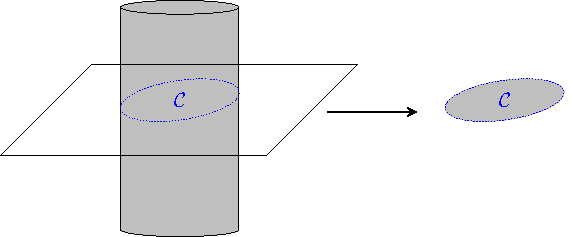
\includegraphics[width=0.8\textwidth]{passive/dimensionReduction.pdf}
 \caption[Schematic view of the reduction of Maxwell's equations from 3D to 2D]
	 {Our set of equations will be valid for infinitely long cylinders of
	  arbitrary cross-sections (shown on the left) and arbitrary physical parameters
	  $\epsilon$ and $\mu$. Our cavities, however, are bidimensional (shown on the right). 
	  The dimension reduction thus consists in postulating independence of the fields
	  and physical and geometrical parameters of the cavity with regards to the longitudinal coordinate 
	  and choosing a particular plane $\partial\Omega$.}
\end{figure}

To this effect, it will be useful to separate the field 
in transverse and longitudinal components. Following \cite{JAC1962,SCH2004b}, 
we suppose the fields can be written as 
  \begin{equation}
    \begin{Bmatrix}\bo{E}(\bo{r}_\perp,z)\\\bo{H}(\bo{r}_\perp,z)\end{Bmatrix} = \begin{Bmatrix}\bo{E}(\bo{r}_\perp)\\\bo{H}(\bo{r}_\perp)\end{Bmatrix}e^{i\beta z}
  \end{equation}
and we will also separate the fields and differential operators in two parts
  \begin{equation}
   \bo{E}(\bo{r}_\perp)= \bo{E}_\perp+E_z\bou{z}; \qquad \nabla=\nabla_\perp + \bou{z}\frac{d}{dz}.
  \end{equation}
Substitution in \eqref{eq:passive.formalism.generalCurlEquations} yields
  \begin{align}
    ik\mu H_z 		&= \left(\nabla_\perp\times\bo{E}_\perp\right)_z			& -ik\epsilon E_z 		&= \left(\nabla_\perp\times \bo{H}_\perp\right)_z	\label{eq:passive.formalism.longitudinalComponents}\\
    ik\mu\bo{H_\perp}	&= \left(-i\beta\bo{E}_\perp+\nabla_\perp E_z\right)\times\bou{z}	& -ik\epsilon\bo{E}_\perp 	&= \left(-i\beta\bo{H}_\perp+\nabla_\perp H_z\right)\times\bou{z} \label{eq:passive.formalism.tranverseComponents}
  \end{align}
The symmetry of these equations allow the decoupling of the tranverse and longitudinal components. 
Solving the system \eqref{eq:passive.formalism.tranverseComponents} 
shows that the scalar components $H_z$ and $E_z$ are the fundamental ones:
  \begin{subequations}
  \begin{align}
    \bo{E}_\perp	&= \frac{i}{k^2n^2-\beta^2}\left[\beta\nabla_\perp E_z+k\mu\nabla_\perp H_z\times\bou{z}\right]	\\
    \bo{H}_\perp	&= \frac{i}{k^2n^2-\beta^2}\left[-k\epsilon\nabla_\perp E_z\times\bou{z}+\beta\nabla_\perp H_z\right].
  \end{align}
  \end{subequations}
Derivation of the differential equation for $E_z$ and $H_z$ can be
done via equations \eqref{eq:passive.formalism.longitudinalComponents}, but
is quite cumbersome. A component-wise approach is thus presented in Appendix \ref{app:basicEquations}. 

More specific boundary conditions can be derived with the use of these equations.
Applying the tranverse and longitudinal decomposition on \eqref{eq:passive.formalism.generalBoundaryConditions}
yields the six boundary conditions
  \begin{align*}
   E_{z1}		&= E_{z2}		& H_{z1}	&= H_{z2}	\label{eq:passive.formalism.contLongComponents}\\
   E_{t1}		&= E_{t2}		& H_{t1}	&= H_{t2}	\\
   \epsilon_1E_{n1}	&= \epsilon_2E_{n2}	& \mu_1H_{n1}	&= \mu_2H_{n2}
  \end{align*}
We seek to write the boundary conditions as a function of $H_z$ and $E_z$,
given that they are the fundamental fields. This can be done by taking
the projections of the transverse fields:
  \begin{subequations}
  \begin{align}
   E_t	&= \bou{t}\cdot\bo{E}_\perp = \frac{i}{\gamma^2}\left[\beta\partial_tE_z-k\mu\partial_nH_z\right]	\\
   E_n	&= \bou{n}\cdot\bo{E}_\perp = \frac{i}{\gamma^2}\left[\beta\partial_nE_z+k\mu\partial_tH_z\right]	\\
   H_t	&= \bou{t}\cdot\bo{H}_\perp = \frac{i}{\gamma^2}\left[k\epsilon\partial_nE_z+\beta\partial_tH_z\right]	\\
   H_n	&= \bou{n}\cdot\bo{H}_\perp = \frac{i}{\gamma^2}\left[-k\epsilon\partial_tE_z+\beta\partial_nH_z\right]	
  \end{align}
  \end{subequations}
where $\partial_{t,n}$ are the transverse and normal derivatives, respectively, and $\gamma^2=k^2n^2-\beta^2$.
Substituting these results in the boundary conditions for the transverse and normal components, we can 
derive the conditions $\partial_tE_{z1}=\partial_tE_{z2}$, $\partial_tH_{z1}=\partial_tH_{z2}$, which can 
shown to be equivalent to the continuity of the longitudinal components, 
\textit{viz.} \eqref{eq:passive.formalism.contLongComponents} \cite{SCH2004b}.
Combining all our previous results yields the four independent 
boundary conditions:
  \begin{subequations}
  \label{eq:passive.formalism.cylindricalBoundaryConditions}
  \begin{align}
   E_{z1}	&= E_{z2}	\\
   H_{z1}	&= H_{z2}	\\
   \frac{k\mu_1}{\gamma_1^2}\frac{\partial H_{z1}}{\partial n}-\frac{k\mu_2}{\gamma_2^2}\frac{\partial H_{z2}}{\partial n} & = \beta\left(\frac{1}{\gamma_1^2}-\frac{1}{\gamma_2^2}\right)\frac{\partial E_{z1}}{\partial t}\\
   \frac{k\epsilon_1}{\gamma_1^2}\frac{\partial E_{z1}}{\partial n}-\frac{k\epsilon_2}{\gamma_2^2}\frac{\partial E_{z2}}{\partial n} & = -\beta\left(\frac{1}{\gamma_1^2}-\frac{1}{\gamma_2^2}\right)\frac{\partial H_{z1}}{\partial t}.
  \end{align}
  \end{subequations}
Notice that the propagation constant couples the electric 
and magnetic fields, regardless of the physical and geometrical
parameters of the cavity. 

\section{Scattering Matrix Formalism}
The previous section has provided us with the differential equations that 
we will need to solve to properly model bidimensional cavities. In this section, 
we will set up a scattering matrix (\gls{sMatrix}) formalism, augmented by the
time-delay matrix \textit{\gls{qMatrix}}
that will allow us to quantify the response of the cavities
to an applied field and provide us with a novel way to determine their resonances. 
The numerical implementation of the method, being somewhat problematic, will 
be discussed at length. 

\subsection{$\mat{S}$ and $\mat{Q}$ Matrices Reloaded}
In dielectric cavities, we need to solve the following equations (see Appendix \ref{sec:app.basicEquationScattering})
  \begin{multline}
    \left\{\nabla^2+k^2n^2\left[1-\left(\frac{\beta}{kn}\right)^2\right]\right\}\begin{Bmatrix} H_z \\ E_z \end{Bmatrix}
      = \frac{1}{1-\left(\frac{\beta}{kn}\right)^2}
	  \left[\frac{1}{\epsilon}\begin{Bmatrix} \nabla H_z \\ \nabla E_z \end{Bmatrix}\cdot\nabla\epsilon+\frac{1}{\mu}\begin{Bmatrix} \nabla  H_z \\ \nabla E_z \end{Bmatrix}\cdot\nabla\mu\right]
      \\-\begin{pmatrix} \frac{1}{\mu} & 0 \\ 0 &\frac{1}{\epsilon}\end{pmatrix} \begin{Bmatrix} \nabla H_z \cdot\nabla\mu \\ \nabla E_z\cdot\nabla\epsilon \end{Bmatrix}
      +\frac{\beta/kn}{1-\left(\frac{\beta}{kn}\right)^2}\left[\left(\sqrt{\frac{\mu}{\epsilon}}+\sqrt{\frac{\epsilon}{\mu}}\right)\begin{pmatrix}0 & -\frac{1}{\mu}\\\frac{1}{\epsilon} & 0\end{pmatrix}
      \begin{Bmatrix} \nabla H_z\times\nabla\mu \\ \nabla E_z\times\nabla\epsilon\end{Bmatrix}\right]
  \end{multline}
where $\beta$ is the propagation constant in the longitudinal direction.
Inhomogeneous cavities do not obey Helmholtz's equation like homogeneous
cavities do, but depend upon the first-order derivatives of the fields and 
physical properties of the medium. The two longitudinal fields
couple through the last term, where an anti-diagonal matrix appears.

%Modes with finite $\beta$ correspond, in the semiclassical limit, to
%rays that spiral up and down the cavity and refract out through 
%the caps \cite{TUR2005}. The cavity modes, the ones we are interested in, 
%are best modeled using $\beta=0$. 

In fact, this set of equations describe the propagation of light 
in optical fibers of arbitrary cross-section and arbitrary
refractive index profiles. However, we are interested in the modes
that are confined on a two-dimensional surface, the cavity modes. 
These modes must be independent of $z$ and we therefore take 
$\beta=0$. This is the main approximation of our model. It has been shown
to hold only approximately in experimental conditions \cite{DUB2008,BIT2010}, 
but we take the resulting equations to be the exact one. This allow a 
simpler analysis for qualitative exploration; quantitative agreement
could be reached via perturbation methods or by using the integral method
we flesh out in Appendix \ref{sec:app.numTools.lippmannSchwinger}. This approximation 
has the much appreciated benefit of decoupling both the field
equations and the boundary conditions (see \eqref{eq:passive.formalism.cylindricalBoundaryConditions}).

Additionally exploiting the fact that we will only consider
non-magnetic media ($\mu=1$, $\epsilon=n^2$), our equation set becomes
  \begin{subequations}
  \label{eq:passive.formalism.fieldEquations}
  \begin{align}
    \left[\nabla^2+k^2n^2\right] H_z	&= \frac{2}{n}\nabla H_z\cdot\nabla n	\label{eq:passive.formalism.TEequation}\\
    \left[\nabla^2+k^2n^2\right] E_z	&= 0. 
  \end{align}
  \end{subequations}
In the following, it will be advantageous to form the field
$\bo{h}=\bo{H}/n$ \cite{DET2009}. This yields the equation
\cite{DET2009, GAP2013a}
  \begin{equation}
   \left[\nabla^2+k^2n^2-\frac{2\left(\nabla n\right)^2}{n^2}+\frac{\left(\nabla^2n\right)}{n}\right]h_z=0 \tag{\ref{eq:passive.formalism.TEequation}'}
   \label{eq:passive.formalism.TEequationPrime}
  \end{equation}
which is nothing but Helmholtz equation with an additional potential term.

\paragraph{The Quantum Connection}
Before putting forward the scattering formalism, it is interesting
to digress a little and explore the connection between the optical 
world and the quantum world. Specifically, the scalar version of
Maxwell's equations, the Helmholtz equations above, can be written 
as a Schrödinger equation
	\begin{equation}
		\left[\nabla^2+k^2\right]\psi = k^2\left(1-n^2(r,\theta)\right)\psi - V(\bo{r})
	\end{equation}
where $V(\boldsymbol{r})$  is the additional potential term just mentioned.
If the r.h.s. is such that equation is amenable to a solution by 
separation of variables, one obtains a radial potential of the form
	\begin{equation}
		V_\text{eff}(r) = k^2(1-n^2(r))+\frac{m^2-1/4}{r^2}.
	\end{equation}
For the example of the homogeneous, circular cavity, this yields a
potential as seen in Figure \ref{fig:passive.formalism.quantumConnection}. 
The jump at the boundary allows the existence of quasi-bound states inside
the cavity, as opposed to bound states, as the light can tunnel outside the
potential barrier.

It is worth mentioning that the TM polarization behaves exactly has a 
quantum wavefunction does, the field and its normal derivative being
continuous at the interface, while the TM polarization is akin to 
a sonorous vibrations, as they may also obey ``jump'' conditions
at an interface \cite{COL2013}. Because of this, the TM polarization
is more present in the E.M. literature than the TE polarization.

\begin{figure}
	\centering
	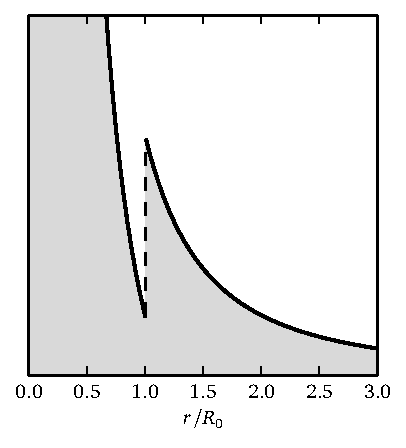
\includegraphics{figs/passive/quantumPotential.pdf}
	\caption[Effective radial potential associated with the homogeneous, circular cavity]
			{Effective radial potential associated with the homogeneous, circular cavity.
			We show the potential for $kR_0=5$, $m=10$ and $n_c=2$.}
	\label{fig:passive.formalism.quantumConnection}
\end{figure}

\begin{figure}
 \centering
 \def\svgwidth{0.4\textwidth}
 \input{figs/passive/dielectric.pdf_tex}
 \caption[Geometry of a bidimensional cavity]
	 {Geometry of a dimensional cavity. $R_0$ is the radius of the smallest circle
	 that encloses the physical microcavity. $R_V$ is the radius of a fictional circle
	 that we will take to go to infinity.}
\end{figure}


To solve these equations, we will adopt a scattering viewpoint. 
Imagine that the dielectric cavity is embedded in an infinite
medium of constant refractive index  $n_o=\sqrt{\epsilon\mu}$, 
outside the cavity, $\bo{r}\not\in{\mathcal{C}}$, 
the r.h.s. of \eqref{eq:passive.formalism.fieldEquations} vanish. 
The resulting equations are Helmholtz's and therefore have the well-known solution
  \begin{equation}
    \label{eq:passive.formalism.hankelSolution}
    \psi = \sum_{m} \left[A_m H_m^{(-)}(nkr) + B_m H_m^{(+)}(nkr)\right]e^{im\theta} \qquad (r>R_0).
  \end{equation}
where $H_m^{(\pm)}(z)$ are the Hankel functions of the first
and second kind. The Hankel functions are chosen in lieu of their
usual homologues $J_m(z)$ and $Y_m(z)$ as their asymptotic forms 
have incoming/outgoing cylindrical wave character, 
$H_m^{(\pm)}\propto \exp(\pm ikr)/\sqrt{r}$, thus ensuring that
Sommerfeld's radiation condition is fulfilled. The scattering
viewpoint essentially describes the relationship between the 
outgoing coefficients, $B_m$, and the incoming coefficients, $A_m$
via the \textit{scattering matrix}
  \begin{equation}
  	\label{eq:passive.formalism.defSmatrix}
    B_m = \sum_{m'}S_{mm'}A_{m'}. 
  \end{equation}
Much like its quantum-mechanical counterpart, the electromagnetic scattering
matrix can be interpreted as a phase shift acquired by the incoming
waves through interaction with the potential. This is most easily seen
by considering a central potential $V(r)$ where the \gls{sMatrix}
is diagonal. In that case, the $m$th component of the far-field can
be written as
  \begin{equation}
   \label{eq:passive.formalism.centralPotentialField}
   \psi_m^\text{FF} \propto \frac{1}{\sqrt{r}}\left[e^{-ikr}+e^{i\delta_m}e^{ikr}\right]
  \end{equation}
where we have written $S_{mm}=e^{i\delta_m}$ with $\delta_m\in\mathbb{R}$ 
as per the unitarity condition. The non-diagonal
generalization $S_{mm'}$ describes the coupling between angular
momenta $m\rightarrow m'$ and can be interpreted as a transition
probability.

When the \gls{sMatrix} is defined by the pair \eqref{eq:passive.formalism.hankelSolution}
and \eqref{eq:passive.formalism.defSmatrix}, it contains all near- and
far-field information. This is sharp contrast with the usual quantum 
scattering matrix, which is usually defined for an \gls{lss} having 
$r\rightarrow\infty$, i.e. in the far-field \cite{NEW1982}. In the scattering off dielectric structures, the potential 
$1-n^2$ has compact support in $\mathbb{R}^d$ and the \gls{lss} is taken to be 
a $(d-1)$-sphere containing the support of the potential.

In most applications (see the Introduction), we wish to find the \textit{resonances} of the
cavity. This is usually done by enforcing Sommerfeld radiation conditions
on Helmholtz's equation and looking for solutions of
  \begin{equation}
   \label{eq:passive.formalism.resonanceCondition}
   \mat{S}^{-1}\bo{B}=0;
  \end{equation}
a solution exists only if $|\det{\mat{S}(k)}|\rightarrow\infty$, 
at a pole of the \gls{sMatrix}. 
For real potentials, there cannot exist a solution on the real $k$ line because
of the flux conservation (unitarity) property of the \gls{sMatrix}. We 
must extend the search to the complex $k$ plane.

Equation \eqref{eq:passive.formalism.resonanceCondition} shows that the cavity 
\textit{creates} energy from nothing. In more physical terms, the cavity
has an infinite response to an infinitesimal energy input. This definition
of a resonance implies that we should look in the $\Im{k}<0$ half-plane
for the poles of the \gls{sMatrix}. The solutions to this equation 
are known as quasi-bound states, as their intensity is usually larger
in the vicinity of the cavity and, contrary to their truly bound counterparts, 
have a small but non-zero value outside it. The ever so slowly decaying wavefunction
is thus non-normalizable (i.e. $\psi\notin L^2$). In this formulation, the field
has the following non-physical behaviour in the far-field
  \begin{align*}
   \psi_\text{FF}(\bo{r},t) 			&= \psi(\bo{r})e^{-i\omega t}	\\
						&\propto \exp\left[i(k'-ik'')\right]\exp\left[-ic(k'-ik'')t\right]\exp[im\theta]	\\
   \left|\psi_\text{FF}(\bo{r},t)\right|^2 	&\propto e^{2k''r}e^{-2ck''t} 
  \end{align*}
where $k=k'-ik''$. The field thus exponentially increases with $r$, 
but exponentially \textit{decreases} with $t$. We can see, however, 
that the time scale of the exponential decrease is linked to the
imaginary part of the wavenumber by $\tau=\left(2k''c\right)^{-1}$.
We will use this relationship later in this essay.

It is interesting to note that the kind of resonances supported
by dielectric cavities are of the same kind as those supported
by a forced, undamped harmonic oscillator. The incoming wave field
plays the part of the applied force. In the treatment of 
harmonic oscillators, it is usually noticed that adding a friction 
term in the equations curbs the infinities that the model otherwise 
yields. A parallel situation occurs in dielectric cavities. When there
is no absorption losses (friction), the response of the cavity 
to an incoming wave field is a result of the cumulative effect 
of the experimentally unattainable complex poles of the scattering matrix. 
However, when losses/gain are added into the model, the poles of the scattering
matrix begin to move in the complex plane; loss of unitarity implies that
it is possible that these poles may eventually move to the real $k$-line, 
making them experimentally possible. This is in fact the backbone 
of the \gls{salt} \cite{GE2010a,GE2010b}.

Instead of directly looking for the poles, we will look for the signatures
of these poles on the real $k$ line by computing the \textit{energy}
of the modes and their complex coupling. This part of the formalism
was initially developed by G.P.-A. \cite{GAP2013a}: we will repeat
only what is necessary. 

Recall that the average electromagnetic energy of a field
in a given volume $V$
  \begin{equation}
   \mathcal{E}^V = \frac{1}{2}\mathop{\iiint}_V\left[\epsilon\bo{E}^*\cdot\bo{E}+\mu\bo{H}^*\cdot\bo{H}\right]d^3\bo{r}.
  \end{equation}
We form the energy matrix 
  \begin{equation}
   \mathcal{E}^V_{mm'} = \frac{1}{2}\mathop{\iiint}_V\left[\epsilon\bo{E}^*_m\cdot\bo{E}_{m'}+\mu\bo{H}^*_m\cdot\bo{H}_{m'}\right]d^3\bo{r}.
  \end{equation}
We will carry out the rest of the computation for the TM mode ($H_z=E_r=E_\theta=0$);
the argument holds for TE polarization \textit{mutatis mutandis} because of the
$k$-independence of the additional potential term in \eqref{eq:passive.formalism.TEequationPrime}
and also because $\bo{h}\propto\bo{H}$ for $r>R_0$. We thus have 
  \begin{align*}
    \bo{E}	&= \psi\bou{z}	\\
    \bo{H}	&= \frac{1}{ik}\nabla\times\bo{E}
  \end{align*}
and the energy matrix becomes
\begin{align}
    \mathcal{E}^V_{mm'}	&= \frac{1}{2}\mathop{\iiint}_V\left[\epsilon\psi^*_{m}\psi_{m'}+\frac{1}{k^2}\left(\nabla\times\psi_{m}\bo{\hat{z}}\right)\cdot\left(\nabla\times\psi^*_{m'}\bo{\hat{z}}\right)\right]d^3\bo{r}.	\nonumber\\
  \end{align}
Taking the parametric derivative of Helmholtz' equation, we get the 
following relations
  \begin{subequations}
  \label{eq:passive.formalism.parametricHelmholtz}
  \begin{align}
   \left[\nabla^2+n^2k^2\right]\psi								&=0	\\
   \left[\nabla^2+n^2k^2\right]\psi^*								&=0	\\
   \nabla^2\frac{\partial\psi}{\partial k}+2kn^2\psi+n^2k^2\frac{\partial\psi}{\partial k}	&=0
  \end{align}
  \end{subequations}
where we assume a real potential.
Forming the product\footnote{We use the identities \cite[Appendix II]{STR41}
  \begin{equation*}
    \nabla\cdot\left(\phi\bo{A}\right) = \bo{A}\cdot\nabla\phi+\phi\nabla\cdot\bo{A}.
  \end{equation*}
and
  \begin{equation*}
    (\bo{a}\times\bo{b})\cdot(\bo{c}\times\bo{d}) = \bo{a}\cdot\left[\bo{b}\times(\bo{c}\times\bo{d})\right].
  \end{equation*}
}
  \begin{align*}
   \frac{1}{2k}\nabla\cdot\left[\frac{\partial\psi}{\partial k}\nabla\psi^*-\psi^*\nabla\frac{\partial\psi}{\partial k}\right]
	&= \frac{1}{2k}\left[\nabla\psi^*\cdot\nabla\frac{\partial\psi}{\partial k}+\frac{\partial\psi}{\partial k}\nabla^2\psi^*
			  -\nabla\frac{\partial\psi}{\partial k}\cdot\nabla\psi^*-\psi^*\nabla^2\frac{\partial\psi}{\partial k}\right]	\\
	&= \frac{1}{2k}\left[n^2\psi^*\left(2k\psi+k^2\frac{\partial\psi}{\partial k}\right)-\frac{\partial\psi}{\partial k}n^2k^2\psi^*\right]\\
	&= n^2\psi^*\psi
  \end{align*}
to write the energy matrix as
  \begin{align*}
    \mathcal{E}^V_{mm'} &= \frac{1}{4k}\int_V\nabla\cdot
			    \left\{
			      \frac{\partial\psi_{m'}}{\partial k}\nabla\psi^*_{m}-\psi^*_m\nabla\frac{\partial\psi_{m'}}{\partial k}
			+   \frac{2}{k}\left[\psi_{m'}\bo{\hat{z}}\times\nabla\times\psi^*_m\bo{\hat{z}}\right]\right\}d^3\bo{r}
  \end{align*}
Using the divergence theorem, noting that the normal vector
is the radial vector, we obtain
  \begin{align*}
    \mathcal{E}^V_{mm'}	&= \frac{wR_V}{4k}
			  \int_0^{2\pi}\left(\frac{\partial\psi_{m'}}{\partial k}\frac{\partial\psi^*_m}{\partial r}
					      -\psi^*_m\frac{\partial^2\psi_{m'}}{\partial k\partial r}\right)d\theta	\nonumber
			+\frac{wR_V}{2k}
			  \int_0^{2\pi}\psi_{m'}\frac{\partial\psi^*_m}{\partial r} d\theta
  \end{align*}
Using the exterior solution for $\psi_m$ and using the 
asymptotic expressions \eqref{eq:app.Bessel.asymptoticHankel} for the Hankel functions, we get
(after some algebra)
  \begin{align}
   \mathcal{E}^{\infty}_{mm'} &= \lim_{R_V\rightarrow\infty}\left[\frac{4n_0wR_V}{k}+\mathcal{O}(R_V^{-1})\right]\delta_{mm'}
			      + \frac{4w}{k}\left(-i\sum_\ell S^*_{\ell m}\frac{\partial S_{\ell m'}}{\partial k}\right)
  \end{align}
where $w$ is the thickness of the cavity. The first term is the 
diverging energy of the beam. Given that the incoming 
and outgoing waves are of infinite extent, this divergence
is only natural. The second term, however, depends only the
potential and can be interpreted as an excess energy due to the
cavity \cite{GAP2013a}. In matrix notation, we have
  \begin{equation}
  	\label{eq:passive.formalism.qMatrixDef}
    \mat{Q} = -i\mat{S}^\dagger\frac{d\mat{S}}{dk}.
  \end{equation}
This result coincides with the \gls{qMatrix} of quantum 
mechanics \cite{SMI1960}. The interpretation of this 
matrix is facilitated by \eqref{eq:passive.formalism.centralPotentialField}. 
Using the central potential, we can write
  \begin{equation}
    Q_{mm} = -ie^{-i\delta_m}\left(i\frac{\partial\delta_m}{\partial k}\right)e^{i\delta_m} = \frac{\partial\delta_m}{\partial k}.
  \end{equation}
The \gls{qMatrix} thus corresponds to the energy derivative of the 
phase shift, which has long been associated with the time-delay
introduced by the potential \cite{EIS1948,SMI1960,CAR2002}. 

The keen reader will have noticed that the above derivation
fails for complex potentials. The author has not found a proper
derivation for the extension to complex potentials. However, 
an expression can be found by this heuristic argument:
when the potential is complex, the phase shift $\delta_m$
becomes a complex function of $k$. In the preceding expression, 
we should take the inverse of the scattering matrix, not its Hermitian
transpose, to reproduce the energy derivative of the phase shift.
We thus have
  \begin{equation}
   \mat{Q} = -i\mat{S}^{-1}\frac{d\mat{S}}{dk}
  \end{equation}
as the proper generalization. This form was also used by Smith in
\cite{SMI1960}.

It is possible to arrive at this result with our derivation, but
with the extra term
	\begin{equation}
		-ik\mathop{\iint}_\mathcal{C}\Im{\epsilon(r,\theta)}\psi_m^*\frac{\partial\psi_{m'}}{\partial k}d^2\bo{r}
	\end{equation}
where $\mathcal{C}$ is the cavity region and the support of 
$\Im{\epsilon(r,\theta)}$. A similar result was obtained in 
\cite{MAR1975} where it was shown that this augmented \gls{qMatrix}
shares some properties of the Wigner-Smith time-delay matrix 
\eqref{eq:passive.formalism.qMatrixDef}. We will derive some of
these properties below. 

\todo[inline]{Discuss the modes defined by the eigenvectors of $Q$.}

\subsection{Properties of the $\mat{S}$ and $\mat{Q}$ matrices}
The $\mat{S}$-matrix has multiple symmetries which can be used 
either to verify numerical implementations or to help tame 
numerical divergence issues. Most of the symmetries we will
expose in this thesis will concern the analytical continuation
of the scattering matrix in the complex $k$ plane. 

It is well known that the $\mat{S}$-matrix is unitary 
for real values of $n$ and $k$ \cite{NEW1982}. However, 
it loses this important property is lost when we extend
to the complex plane. Looking at the complex conjugated versions
of our equation set, we see that we have
  \begin{align*}
    B_m		&= S_{mm'}(n,k)A_{m'}	\\
    A_m^*	&= S_{mm'}(n^*,k^*)B_{m'}^*
  \end{align*}
we can obtain the relation
  \begin{equation}
    \label{eq:passive.formalism.generalizedSmatrix}
    \mat{S}^{-1}(n^*,k^*) = \mat{S}^\dagger(n,k)
  \end{equation}
which reduces to the unitarity condition when 
the values are real. 

\begin{figure}
 \centering
 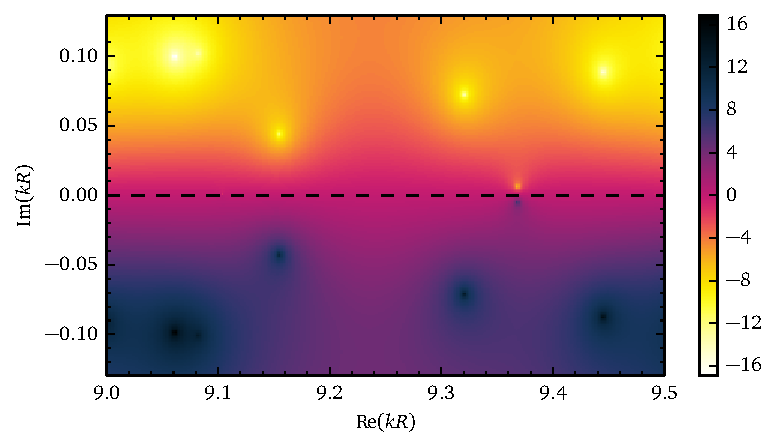
\includegraphics[width=0.8\textwidth]{figs/passive/determinantSmatrix.pdf}
 \caption[Mirror symmetry of the scattering matrix]
	 {Mirror symmetry of the scattering matrix. For this example, 
	 we computed $\log\det\mat{S}(k)$ for the scattering matrix of the
	 circular, homogeneous cavity with $n_c=3.2$ and $n_o=1$.}
  \label{fig:passive.formalism.symmetrySmatrix}
\end{figure}

Following \cite{GAP2013a}, we set up the following scattering
``experiment'':
  \begin{align*}
    H_m^{(-)}(z)e^{im\theta}					&\rightarrow \sum_{m'} S_{m'm}(n,k)H_{m'}^{(+)}(z)e^{im'\theta}	\tag{initial reaction}\\
    \sum_{m}S_{m'm}^*(n^*,k^*)H_m^{(-)}(z)e^{im\theta}		&\rightarrow H_{m'}^{(+)}(z)e^{im'\theta}			\tag{relation \eqref{eq:passive.formalism.generalizedSmatrix}}\\
    \sum_{m}S_{m'm}(n^*,k^*)\overline{H_m^{(-)}(z)}e^{-im\theta}&\leftarrow \overline{H_{m'}^{(+)}(z)}e^{-im'\theta}.		\tag{complex conjugate (time reversal)}
  \end{align*}
Use of \eqref{eq:app.Bessel.conjHankel}
leads to the relation, valid only when $k\in\mathbb{R}$
  \begin{equation}
    \label{eq:passive.formalism.timeReversalSymmetryReal}
    S_{m'm}(n,k) = (-1)^{m'}S_{-m-m'}(n^*,k)(-1)^m.
  \end{equation}
This relationship will be incredibly useful in the numerical implementation.

The \gls{qMatrix} also has some interesting properties. For real
potentials, it is Hermitian. This is a direct consequence of the
unitarity of the \gls{sMatrix} as 
  \begin{equation}
   \frac{d\mat{S}^\dagger\mat{S}}{dk} = \frac{d\mat{S}^\dagger}{dk}\mat{S}+\mat{S}^\dagger\frac{d\mat{S}}{dk} = 0
  \end{equation}
and
  \begin{equation}
   \mat{Q}^\dagger = i\frac{d\mat{S}^\dagger}{dk}\mat{S} = -i\mat{S}^\dagger\frac{d\mat{S}}{dk} = \mat{Q}
  \end{equation}
The delays associated with the potential are thus always real
and the delay eigenstates form a complete basis. Perhaps the
most interesting, and important, result concerning the 
\gls{qMatrix} is its connection with the complex poles of the
scattering matrix. It can be shown (see \cite{SHI2011,SHI2012,GAP2013a})
that we can seperate the scattering matrix in \textit{resonance channels} $\{\ket{p_j}\}$
and arrive at Simonius' form \cite{SIM1974}
  \begin{equation}
   \mathbf{S}(k)=\prod_{j=1}^\infty \mathbf{S}_j(k)
  \end{equation}
where
  \begin{equation}
   \mat{S}_j(k)\Ket{p_j} = \frac{k-k_j^*}{k-k_j}\Ket{p_j}.
  \end{equation}
Notice that this unitary expansion on the basis of the resonance
channels contains the mirror-symmetry of the poles and zeros of the 
scattering matrix. Figure \ref{fig:passive.formalism.symmetrySmatrix}
shows this symmetry in the case of the scattering matrix of the circular
disk. 

Using Simonius' expansion and the definition of the \gls{qMatrix}, we can obtain that
the eigendelays $q_p$ of each resonance channel have the form
  \begin{equation}
   \label{eq:passive.formalism.lorentzianDelays}
   q_p \propto \sum_j \frac{\Gamma_j}{\left(k-\Re{k_j}\right)^2-\Gamma_j^2/4}
  \end{equation}

In the complex case, things become more complicated. Simonius' 
expansion is no more valid, as the poles and zeros are not 
longer symmetric along the real axis. The symmetry line
is shifted upward in the complex plane \cite{SAV2003,FYO2005}. 
Evaluating the \gls{qMatrix} along this line yields
a spectrum of real eigenvalues, referred to as the proper delay times. 
However, when the absorption is dispersive, the amount by which the symmetry
line depends on $\Re{k}$. We must thus evaluate the \gls{qMatrix} along
a curve in the complex $k$-plane. This shift depends non-trivially
on the absorption. It thus becomes rather hard to extract any meaningful
information for the \gls{qMatrix} for a general, complex, potential. 

The \gls{sMatrix} also suffers some dramatic changes in its pole structure
\cite{JOF1973,KOK1981}, but the fact remains that the poles can still be
interpreted as the resonances of the cavity, and that the complex positions
yield information about the lifetimes of those resonances. Taking everything
into consideration, it seems that, for complex potentials, it is easier to 
work directly with the scattering matrix than to deal with the \gls{qMatrix}.

\section{Numerical Implementation}
The numerical computation of the scattering matrix 
depends on two constructs: a polar discretization 
scheme and interior scattering matrices. We choose, for
the former, a rather standard radial discretization 
(see Fig. \ref{fig:passive.numerical.radialDiscretization}).
For easier reference, we dub the method \gls{sqa}.

\begin{figure}
 \centering
 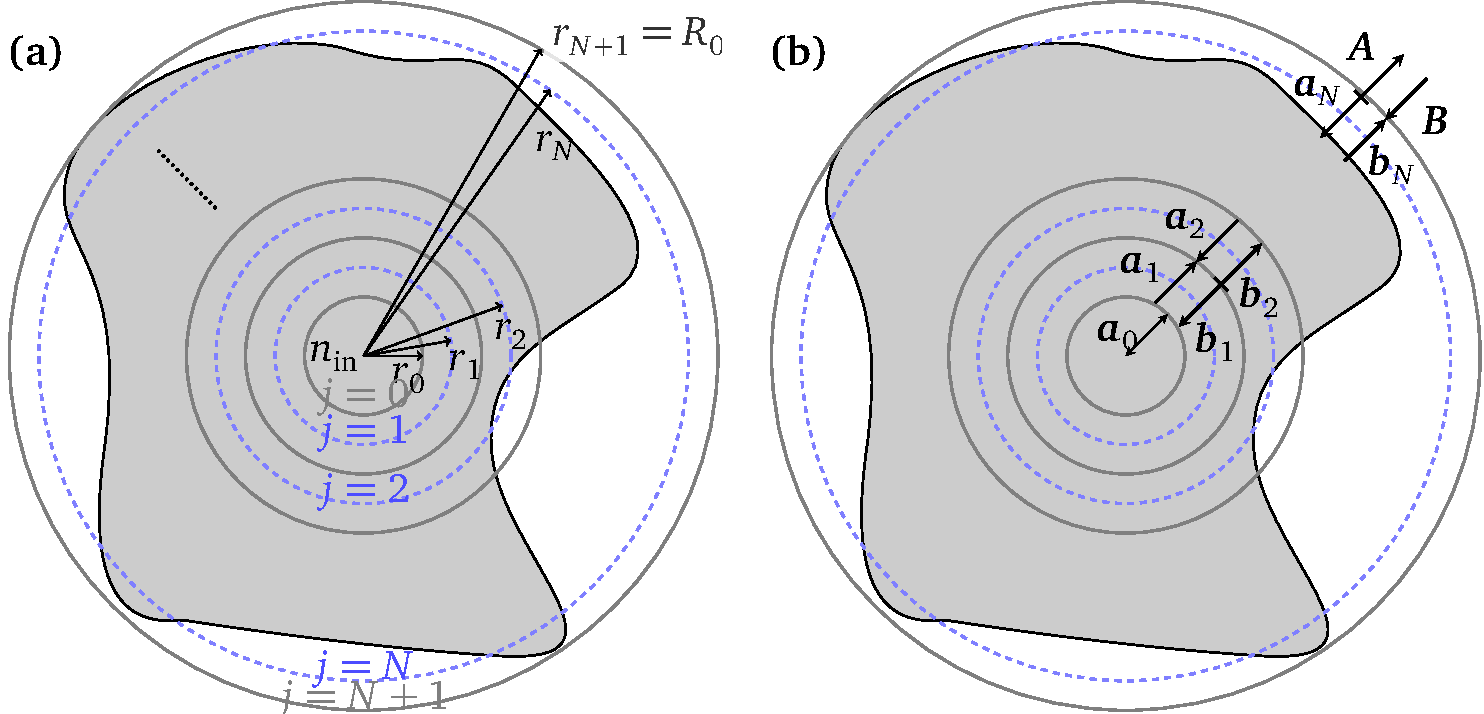
\includegraphics[width=0.9\textwidth]{figs/passive/figDisScatCoeff.pdf}
 \caption[Radial discretization for use in SQA]
	 {Radial discretization of the cavity for use in \gls{sqa}. The inner circle is assumed to 
	 have a constant refractive index denoted $n_\text{in}$. The full grey lines represent
	 the physical boundaries of each shell while the dotted blue lines represent their
	 center. \textbf{(a)} The central radius $r_j$ is the radial position at which the 
	 refractive index is sampled. Theh boundary conditions are enforced at $r=r_j\pm\epsilon$.
	 \textbf{(b)} Note the alternating propagation directions of the solutions inside each shell.
	 This reflects the local definition of ``incoming'' vs ``outgoing waves'' for each $r_j$.}
  \label{fig:passive.numerical.radialDiscretization}
\end{figure}

The latter relate the solutions of the differential equation 
inside each radial shell to its neighboring shell. The final
interior scattering matrix relates the solution in the last shell
to the exterior solution, which is analytically known and is 
related to the \gls{sMatrix}\index{scattering matrix} of the cavity.

Our method is based on an algorithm originally developed by 
Rahachou and Zozoulenko \cite{RAH2004} and extended by \cite{GAP2013a}. 
We generalize the method to accept complex refractive index
profiles $n$ and wavenumbers $k$. 

\subsection{\textit{Divide et impera}}
We wish to solve the Helholtz equation 
  \begin{equation}
   \left[\nabla^2+k^2n^2\right]\psi = 0
  \end{equation}
inside the cavity. For $r>R_0$, the radius of the smallest circle
that encloses the whole dielectric, the solution is 
\eqref{eq:passive.formalism.hankelSolution}. We apply the discretization
of Fig. \ref{fig:passive.numerical.radialDiscretization}. We define a set of 
radii $\left\{r_j\right\}_{j=0}^{N+1}$ that denote the positions of the center
of the different shells. As such, $r_j-r_{j-1}=2\epsilon$ for the inner shells.
The cases $j=0$ and $j=N+1$ are different in that $r_0$ and $r_{N+1}$ denote 
the outer and inner limits of the domains, respectively. Moreover, $r_{N+1}-r_N=r_1-r_0=\epsilon\neq2\epsilon$.
As our first approximation, we suppose that the refractive index
inside the inner circle is constant and call it $n_\text{in}$. The Helmholtz equation then merely
becomes the Bessel equation \eqref{eq:app.Bessel.diffEquation}. Enforcing
finiteness of the field at $r=0$, we have the solution
  \begin{equation}
   \Ket{\psi(r)} = \sum_{m}2a_m^0J_m(n_\text{in}kr)\Ket{\Phi_m^0}	\qquad (r<r_0)
  \end{equation}
where we have introduced bra-ket notation for the angular part of the 
solution. In that case, 
  \begin{equation}
   \Braket{\theta|\Phi_m^0} = e^{im\theta}.
  \end{equation}
In the shells $j>0$, the differential equation to solve is rather
  \begin{equation}
    \label{eq:passive.formalism.shellDiffEquation}
    \left[\frac{d^2}{dr^2}+\frac{1}{r}\frac{d}{dr}+\frac{1}{r^2}\frac{d^2}{d\theta^2}+k^2n^2(r,\theta)\right]\psi=0.
  \end{equation}
Inside each shell, we suppose that the potential strength depends only on the angular variable, i.e.
$k^2r^2n^2(r,\theta)\mapsto k^2r_j^2n^2(r_j,\theta)$ such that the angular sampling of the refractive
index is done at $r=r_j$ for each shell. \eqref{eq:passive.formalism.shellDiffEquation} 
is then amenable to a separation of variables
  \begin{subequations}
  \begin{align}
   \left[\rho_j^2\frac{d^2}{d\rho_j^2}+\rho_j\frac{d}{d\rho_j}-\xi^j\right]\mathcal{R}^j	&=0	\label{eq:passive.formalism.radialDiffEqn}	\\
   \left[\frac{d}{d\theta^2}+\left(k^2n^2(r_j,\theta)r_j^2+\xi^j\right)\right]\Phi^j		&=0
  \end{align}
  \end{subequations}
where $\rho_j=r/r_j$ is the scaled radial variable of the shell. 
These equations can readily be solved by noticing that
$\Phi^j(\theta+2\pi)=\Phi^j(\theta)$. We expand the solution
in a Fourier series
  \begin{equation}
   \Braket{\theta|\Phi_\mu^j} = \frac{1}{\sqrt{2\pi}}\sum_{m=-\infty}^\infty c_{m\mu}^je^{im\theta}
  \end{equation}
Projecting onto $\Ket{\Phi_m'^0}$ yields
\begin{equation}
    \sum_{m=-\infty}^\infty\left[-m^2\Braket{\Phi_{m'}^0|\Phi_m^j}+\xi^j\Braket{\Phi_{m'}^0|\Phi_m^j}+k^2r_j^2\Braket{\Phi_{m'}^0|n^2(r_j,\theta)|\Phi_m^j}\right]=0
  \end{equation}
Noticing that 
  \begin{equation}
    \Braket{\Phi_{m'}^0|\Phi_{m}^j} = \sum_{m=-\infty}^\infty c_{m\mu}^j \delta_{mm'}
  \end{equation}
we can write
  \begin{equation}
    \sum_m\left[-m^2\delta_{mm'}+\xi^j\delta_{mm'} + \frac{k^2r_j^2}{2\pi}\int_{0}^{2\pi}n^2(r,\theta)e^{i(m-m')\theta}d\theta\right]c_{m\mu}^j =0.
  \end{equation}
Using this last equation, we can set up an eigenvalue 
problem for the separation constant and the Fourier coefficients
  \begin{equation}
   \label{eq:passive.numerical.eigenvalue}
   \mat{L}^j\bo{c}_\mu^j=\xi_\mu^j\bo{c}_\mu^j
  \end{equation}
with
  \begin{equation}
    L_{mm'}^j = m^2\delta_{mm'}-\frac{k^2r_j^2}{2\pi}\int_0^{2\pi}n^2(r_j,\theta)e^{i(m-m')\theta}d\theta.
  \end{equation}
The particular form and additional properties of this matrix are discussed in 
Appendix \ref{sec:app.numTools.scatMat}.

Now that we know the set of eigenvalues $\{\xi_\mu^j\}$, we can solve the radial
equation \eqref{eq:passive.formalism.radialDiffEqn}. It is instantly recognized as 
a Cauchy-Euler equation. Given its coefficients, one can write the solution 
as \cite[p.~118-119]{GRE98}
  \begin{equation}
    \label{eq:sMatrix.radialSolution}
    \mathcal{R}_\mu^j(r) =  a_\mu^j\rho_j^{+\sqrt{\xi_\mu^j}}+b_\mu^j\rho_j^{-\sqrt{\xi_\mu^j}}.
  \end{equation}
  
Solving the $N$ eigenvalue problems \eqref{eq:passive.numerical.eigenvalue} gives
the solution in all space. We can now apply the boundary conditions \eqref{eq:passive.formalism.cylindricalBoundaryConditions}
at the interface of each shell $j\rightarrow j+1$. The process generates two sets of equations
  \begin{subequations}
  \begin{align}
   \sum_\mu\left[a_\mu^j\rho_j^{+\sqrt{\xi_\mu^j}}+b_\mu^j\rho_j^{-\sqrt{\xi_\mu^j}}\right]\Ket{\Phi_\mu^j}
   &=
   \sum_\mu\left[b_\mu^{j+1}\rho_{j+1}^{+\sqrt{\xi_\mu^{j+1}}}+a_\mu^{j+1}\rho_{j+1}^{-\sqrt{\xi_\mu^{j+1}}}\right]\Ket{\Phi_\mu^{j+1}}	\\
   \eta_j\frac{d}{dr}\sum_\mu\left[a_\mu^j\rho_j^{+\sqrt{\xi_\mu^j}}+b_\mu^j\rho_j^{-\sqrt{\xi_\mu^j}}\right]\Ket{\Phi_\mu^j}
   &=
   \eta_{j+1}\frac{d}{dr}\sum_\mu\left[b_\mu^{j+1}\rho_{j+1}^{+\sqrt{\xi_\mu^{j+1}}}+b_\mu^{j+1}\rho_{j+1}^{-\sqrt{\xi_\mu^{j+1}}}\right]\Ket{\Phi_\mu^{j+1}}
  \end{align}
  \end{subequations}
where $\eta_j = 1\, (1/n(r_j,\theta))$ in TM (TE) polarization. The interior scattering matrices
are constructed via pre-multiplying by the left eigenvectors $\Bra{\tilde{\Phi}_\mu^j}$ on each side. 
Combining both resulting equations leads to the linear system 
  \begin{equation}
    \begin{pmatrix}\mat{A} & \mat{B} \\ \mat{C} & \mat{D} \end{pmatrix} \begin{pmatrix} \bo{a}^j \\ \bo{a}^{j+1}\end{pmatrix}
    =
    \begin{pmatrix}\mat{E} & \mat{F} \\ \mat{G} & \mat{H} \end{pmatrix} \begin{pmatrix} \bo{b}^j \\ \bo{b}^{j+1}\end{pmatrix}
  \end{equation}
which can be inverted using Schur's complements \cite[p.~123]{MEY2001} to yield a relationship between the 
$\bo{a}$ and $\bo{b}$ coefficients, i.e.
  \begin{equation}
   \mat{S}_j = \begin{pmatrix}\mat{E} & \mat{F} \\ \mat{G} & \mat{H} \end{pmatrix}^{-1}\begin{pmatrix}\mat{A} & \mat{B} \\ \mat{C} & \mat{D} \end{pmatrix}.
  \end{equation}
Physically, the $\mat{S}_j$ matrix relates the locally 
incoming waves from shell $j+1$ in shell $j$ to the locally 
outgoing from shell $j$ to shell $j+1$. The last necessary
breakthrough is to realize that we can connect the solutions
from shell $j$ to those of the shell $j+2$, then $j+3$ and 
so on. When started from $j=0$, this iterative process yields
the relationship
  \begin{equation}
   \begin{pmatrix}\bo{a}^0\\\bo{B}\end{pmatrix} = \mat{S}^{0,N}\begin{pmatrix}\bo{a}^0\\\bo{A}\end{pmatrix}
  \end{equation}
such that the \gls{sMatrix} of the system is
the block $\mat{S}_{22}^{0,N}$. More details can be found
in Appendix \ref{sec:app.numTools.scatMat}. 
  
\subsection{Numerical Analysis and Calibration}
While numerical analysis has been heavily formalized in recent years, 
it is still as much an art as a science. In implementing the algorithm, 
we thus came across two potential problems: the inversion of the 
$\mat{K}$ matrix (defined below) and the final Hadamard product
$\mathcal{H}\circ\mat{S}^{0,N}_{22}$. We analyze the two issues
and provide solutions to the instabilities they cause. We also 
calibrate the method with systems whose analytical solution
is known: the homogeneous circular cavity and the annular cavity.
We also compare our method to results obtained in the literature. 

\subsubsection{Numerical Back and Forth}
For the computation of each $\mat{S}_j$, we must invert
a matrix of the form 
  \begin{equation}
  \mat{K}^{j,j+1} = \left(\frac{r_j-\epsilon}{r_j+\epsilon}\right)^{\bo{\Lambda}^j}
		    -\tilde{\mat{S}}^{j+1}_{11}\left(\frac{r_j+\epsilon}{r_j-\epsilon}\right)^{\bo{\Lambda}^j}\tilde{\mat{S}}^{0,j}_{22}.
  \end{equation}
Given that the elements of this matrix highly depend upon the discretization
parameter $\epsilon$, the half-width of the shells, we can use the
condition number $W$ of this matrix as an indicator of the quality
of the discretization. It can be grossly estimated by the 
ratio of the maximum and minimum elements of the matrix. 
By assuming that there is no amplification in the system,
all interior scattering matrices have
$||\mat{S}||<1$ and we can approximate
  \begin{equation}
   W \sim \left(\frac{r_j+\epsilon}{r_j-\epsilon}\right)^{2\lambda_\text{max}}\sim 1 + \frac{4\lambda_\text{max}\epsilon}{r_j}
  \end{equation}
according to the binomial expansion.
To evaluate the $\lambda_\text{max}$ parameter, we will
have to take a detour and introduce the concept 
of \textit{\glspl{gerschgorin}}.

\paragraph{Gerschgorin Circles}
Gerschgorin circles provide a way to bound the spectrum 
of square matrices by simply examining its entries.

\begin{thm}[Gerschgorin circles \protect{\cite[p.~498]{MEY2001}}]
 The eigenvalues of a matrix $\mat{A}\in\mathbb{C}^{n\times n}$ are
 contained within the intersection $\mathcal{G}_r\cap\mathcal{G}_c$
 of the sets of row and column Gerschgorin circles, defined respectively as
  \begin{align*}
   \mathcal{G}_r	&= \left\{|z-a_{ii}| \leq \sum_{\stackrel{j=0}{j\neq i}}^{n-1} |a_{ij}|; \quad \forall i\right\}
  & \mathcal{G}_c	&= \left\{|z-a_{jj}| \leq \sum_{\stackrel{i=0}{i\neq j}}^{n-1} |a_{ij}|; \quad \forall j\right\},
  \end{align*}
 or, in a slightly more algorithmically-friendly form:
  \begin{equation}
   \mathcal{G}_r\cap\mathcal{G}_c = \left\{|z-a_{ii}| \leq \min\left(\sum_{\stackrel{j=0}{j\neq i}}^{n-1} |a_{ij}|,\sum_{\stackrel{j=0}{j\neq i}}^{n-1} |a_{ji}|\right)
				     ;\quad \forall i\right\}.
  \end{equation}
\end{thm}

\begin{corr}\label{corr:passive.numerical.diagDominantMatrices}
 Diagonally dominant matrices are non-singular.
\end{corr}

 \begin{proof}
  Diagonally dominant matrices, by definition, have 
    \begin{equation}
     |a_{ii}| > \max\left(\sum_{\stackrel{j=0}{j\neq i}}^{n-1} |a_{ij}|, \sum_{\stackrel{j=0}{j\neq i}}^{n-1} |a_{ji}|\right)
    \end{equation}
  and, by Gerschgorin's theorem, do not have 0 as an eigenvalue, $0\notin\sigma(\mat{A})$, and therefore are 
  non-singular.
 \end{proof}

\begin{exmp}
  Consider the matrix \cite[p.~499]{MEY2001}
  \begin{equation}
    \label{eq:passive.numerical.exampleMatrixGerschgorin}
    \mat{A} = \begin{pmatrix} 5 & 1 & 1 \\ 0 & 6 & 1 \\ 1 & 0 & -5 \end{pmatrix}.
  \end{equation}
  Its associated Gerschgorin circles are shown in Figure \ref{fig:passive.numerical.gerschgorinCircles}. 
  We see that the row and column circles give different bounds on the eigenvalues and their intersection 
  yields the best possible approximations for the eigenvalues. 
\end{exmp}

\begin{figure}
 \begin{subfigure}{\textwidth}
  \centering
  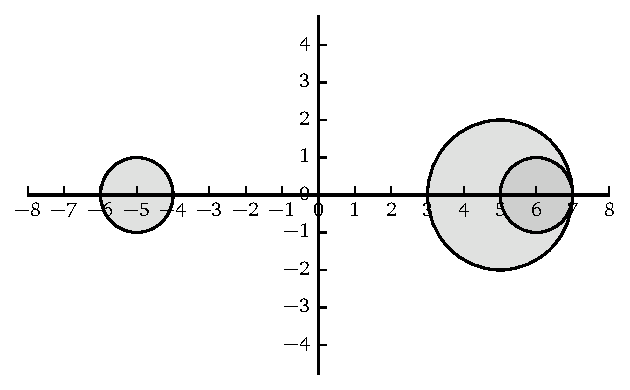
\includegraphics{figs/passive/gerschgorin-row.pdf}
  \caption{Row Gerschgorin circles}
 \end{subfigure}
 
 \begin{subfigure}{\textwidth}
  \centering
  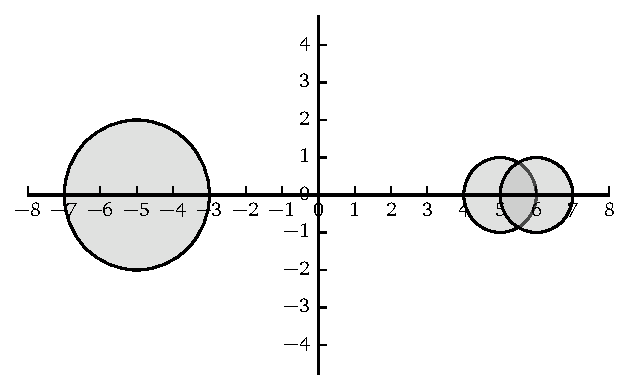
\includegraphics{figs/passive/gerschgorin-col.pdf}
  \caption{Column Gerschgorin circles}
 \end{subfigure}
 
 \begin{subfigure}{\textwidth}
  \centering
  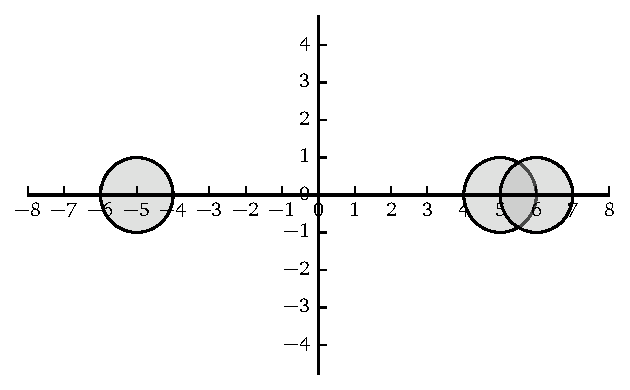
\includegraphics{figs/passive/gerschgorin-full.pdf}
  \caption{Intersection of both previous sets}
 \end{subfigure}
 \caption[Gerschgorin circles for an example matrix]
	 {Gerschgorin circles of the matrix defined in \eqref{eq:passive.numerical.exampleMatrixGerschgorin}.
	 Notice that the matrix is non-singular by Corrolary \ref{corr:passive.numerical.diagDominantMatrices}.}
 \label{fig:passive.numerical.gerschgorinCircles}
\end{figure}

We now apply the Gerschgorin circles to our $\mat{L}^j$ matrix. 
In Appendix \ref{sec:app.numTools.scatMat}, we show that a proper choice for $M$
is $M=2kR_0\sqrt{\mathop{\max}_{(r,\theta)}\left(n^2(r,\theta)\right)}$. This criterion
ensures that we sample the refractive index above the Nyquist frequency. The largest
diagonal element (the farthest Gerschgorin circle) corresponds
to the highest angular momentum and has a magnitude of 
$4k^2R_0^2\mathop{\max}_{(r,\theta)}\left(n^2(r,\theta)\right)-k^2R_0^2n^2(r,\theta)\sim3k^2R_0^2n^2$.
The radius is more complicated to estimate, as it is given by the sum of the norm
of the Fourier coefficients of $n^2(r,\theta)$, which we call $n_m$:
  \begin{equation}
   r = \sum_{m=1}^M |n_m|.
  \end{equation}
It can be shown that there exists an upper bound for the value of the
Fourier coefficients \cite{JAC1920}
  \begin{equation}
   |n_m| \leq \frac{V}{2m\pi}
  \end{equation}
where $V$ is the variation of the refractive index and is define as
  \begin{equation}
   V(r) = \int_0^{2\pi}\left|\partial_\theta n^2(r,\theta)\right|d\theta.
  \end{equation}
To go further, we must realize the mixed blessing of the logarithmic
divergence of the harmonic series\footnote{A better bound could be obtained, but requires conditions
on the behaviour $n^2(r,\theta)$ that the author is not comfortable assuming.}. We estimate the radius
of the Gerschgorin circle by taking $M=500$, an arbitrary bound
that is unattainable by our algorithm\footnote{The Bessel functions overflow our floating representation at approximately $M\sim250$,
rendering the algorithm useless.}
such that the upper bound for the radius becomes $r\leq 3V/\pi$. Taking the annular
cavity as an example, the variation is approximately given by 
$2n^2$. Pulling everything together, this yields an approximate upper
bound for the largest eigenvalue as
  \begin{equation}
   |\lambda_\text{max}| < 3nkR_0
  \end{equation}
A good choice of $\epsilon$ is thus
  \begin{equation}
   \epsilon \ll \frac{1}{12nk} \ll \frac{\lambda}{2n}
  \end{equation}
which mirrors the conventional wisdom. This empirical rule
is applied in every computation in this thesis.

\subsubsection{Hadamard Product}
Like Frodo before Mount Doom, we must face a final challenge
before conquering upon all evil, or, in our case, computing
the scattering matrix. Our final demon
takes the form of the product
  \begin{equation}
   \mat{S} = \left[\mat{H}^{(+)}\right]^{-1}\mat{S}^{0,N}_{22}\mat{H}^{(-)}
  \end{equation}
where the $\mat{H}$ are diagonal matrices with entries $H_m^{(\pm)}(n_okR_0)$. 
We recast the matrix product as a Hadamard (element-wise) product
 \begin{equation}
  \mat{S} = \mathcal{H}\circ\mat{S}^{0,N}_{22}
 \end{equation}
with $\mathcal{H}_{mm'} = H_m^{(-)}(n_okR_0)/H_{m'}^{(+)}(n_okR_0)$.
A quick peek at Fig. \ref{fig:passive.numerical.hankelHadamard} 
announces the disaster. The region $|m'|>|m|$ increases 
exponentially with $|m'|-|m|$. This wouldn't be an issue 
if the corresponding elements of the block scattering
matrix $\mat{S}^{0,N}_{22}$ were exponentially decreasing (as
we physically expect them to); however, the numerical construction
of this matrix implies the addition and subtraction of $\mathcal{O}(1)$
floating-point numbers, limiting their range to about $10^{-15}$, the decimal
accuracy associated with \texttt{double} precision arithmetic. Consequently, 
the final Hadamard product yields scattering matrices with unphysically
large off-diagonal elements.

\begin{figure}
 \centering
 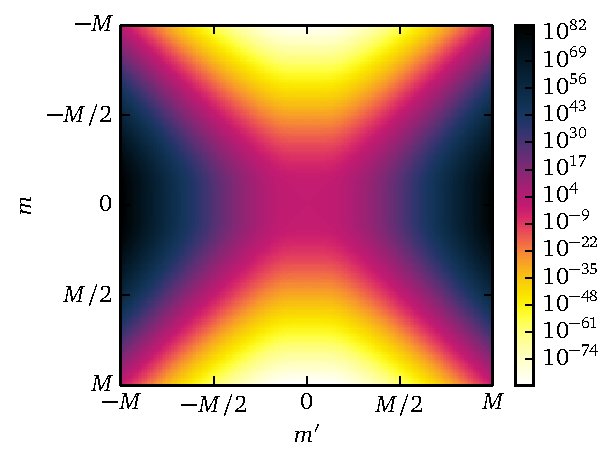
\includegraphics{figs/passive/absHadamard.pdf}
 \caption[General form of absolute value of the Hankel matrix $\mathcal{H}$]
	 {General form of absolute value of the Hankel matrix $\mathcal{H}$.
	 We have used the parameters $z=10$ and $M=100$, but
	  the pattern scales with $M$ and $z$.}
 \label{fig:passive.numerical.hankelHadamard}
\end{figure}

Several solutions to this numerical artefact have been considered, e.g. the use of matrix masks
and of higher precision arithmetic. The latter was swiftly abandoned
due to the difficulty of the implementation\footnote{Even if we disregard
the fact that no C++ compiler support the IEEE 754 \texttt{binary128}
quadruple precision float-point representation, we would still need
to find numerical libraries that extend the BLAS and LAPACK libraries
to work at higher precision.}, even though it could help stabilize the
numerical algorithm \cite[\S 5.8.4]{MIS2002}. The use of matrix masks is 
made possible by noting that the cavity cannot convert arbitrarily
high angular momenta. The maximum angular momentum it can affect, 
$M_\text{max}$ is a function of its ``degree of inhomogeneity'', 
characterized by the absolute size of the Fourier components
of the refractive index (which also depends on the geometry
of the cavity). This gives the \gls{sMatrix} a banded form 
(see Fig. \ref{fig:passive.numerical.bandedFormSmatrix} for
an example using the elliptical cavity). The width of
this band could be detected in $\mat{S}^{0,N}_{22}$ before
taking the Hadamard product, or inferred from the coefficients
of the Fourier transform of $n^2(r,\theta)$. After the product, all elements
outside this band could be set to zero. The interested 
reader might want to go through Türeci's discussion of
the banded form and the numerical problems associated 
with the Hankel matrices \cite[\S 3.4]{TUR2003}.

\begin{figure}
 \centering
 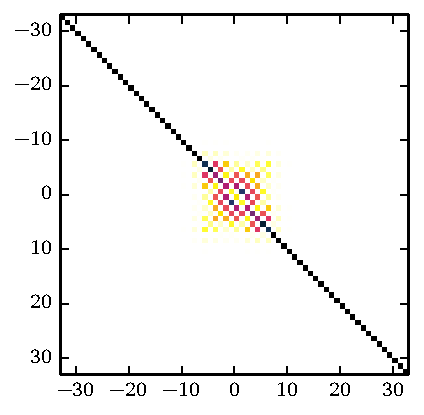
\includegraphics{figs/passive/sMatrixEllipseMag.pdf}
 \caption[Banded form of the scattering matrix of the elliptical cavity]
	 {Scattering matrix of the elliptical cavity with $n_c=3.3$, $a=1$
	 and $b=0.53477$, giving $e=0.845$. Recall that $r(\theta)=ab/\sqrt{(b\cos\theta)^2+(a\sin\theta)^2}$.
	 Notice that the non-vanishing elements have a banded form: they decrease with the distance
	 from the diagonal and eventually go to zero. Beyond a particular value of the angular momentum 
	 ($M_\text{max}=6$, in this case), the scattering matrix is diagonal: there is no mixing of angular momenta.
	 The value of $M_\text{max}$ depends on the inhomogeneity of both the boundary of the cavity and that of its
	 refractive index. It could be inferred from the Fourier transform of the refractive index.}
 \label{fig:passive.numerical.bandedFormSmatrix}
\end{figure}

We have, however, chosen a different path. 
It turns out that relation \eqref{eq:passive.formalism.timeReversalSymmetryReal}
precisely relates the diverging parts of the Hankel matrix
to its vanishing one. Imposing this symmetry on the numerical scattering
matrix allows the algorithm to return physical scattering matrices. 
This limits the scope of our method to real energies ($k$) and has a
high computational cost for complex refractive indices. This limitation, 
coupled to the fragility of the generalization to $n\in\mathbb{C}$ suggests
the use of other methods for complex energies and potentials (see next chapter).

\subsubsection{Calibration}
One of the most important step in algorithmic creation
is the \textit{\gls{calPhase}}. Ours was calibrated
against two cavities: the homogeneous circular cavity and 
the annular cavity. Their analytical form is given below.
We will use 
  \begin{equation}
   E = \max\left[\mat{S}_\text{ana}-\mat{S}_\text{SQA}\right] 
  \end{equation}
as a function of the discretization size $kR_02\epsilon$ to measure
the error. 

\paragraph{Homogeneous, Circular Cavity}
The scattering matrix of the homogeneous circular cavity
is trivially obtained. Assuming that the refractive index inside
the cavity is $n_c$ and $n_o$ outside, the solution inside the 
cavity is given by 
  \begin{equation}
   \psi^c = \sum_m a_m^cJ_m(n_okr)e^{im\theta}
  \end{equation}
while the solution outside the cavity is given by \eqref{eq:passive.formalism.hankelSolution}.
Imposing the electromagnetic boundary conditions yields two infinite sets of equations
for three sets of coefficients. Solving yields a linear relationship between the 
$A_m$ and $B_m$ sets, \textit{viz.} the scattering matrix
  \begin{equation}
   \label{eq:passive.numerical.sMatrixHomo}
   S_{mm'}^\text{HD} = -  \frac{\eta_{co}J_m'(Z_c)H_m^{(-)}(Z_o)-J_m(Z_c){H^{(-)}_m}'(Z_o)}
				{\eta_{co}J_m'(Z_c)H_m^{(+)}(Z_o)-J_m(Z_c){H^{(+)}_m}'(Z_o)}\delta_{mm'}.
  \end{equation}
where $Z_c = n_ckR_0$, $Z_o=n_okR_0$ and $\eta_{co}= n_c/n_o\; (n_o/n_c)$ in TM (TE) polarization.

Before, we showed the correspondence between the poles of the scattering matrix and its associated
time delay spectrum analytically (see p.~\pageref{eq:passive.formalism.lorentzianDelays}). 
In Fig.~\ref{fig:passive.numerical.correspondanceRoots}, we show the
time delay spectrum of the homogeneous disk. The corresponding poles of the \gls{sMatrix} are denoted
by squares\footnote{The poles are computed via the zeros of the denominator of \eqref{eq:passive.numerical.sMatrixHomo}
using a Newton-Raphson algorithm. The initial guesses are provided by the asymptotic ($kR_0\gg m$) zeros
of the denominator. See \cite[Annexe A.2.4]{GAG2011} for a derivation.}. There seems to be a problem with the very high-$Q$ ones, but this is only due to the fact
that we have not used a proper discretization $\Delta k$. The other ones line up perfectly with the peaks
of the time delay. 

In Fig.~\ref{fig:passive.numerical.convergenceHomogeneousDisk}, we compare the analytical scattering
matrix to the one computed via SQA. Notice that the convergence speed is the same for all curves, 
regardless of the value of $kR_0$. Convergence does not depend on the value of $M$
as the homogeneous, circular cavity has a diagonal scattering matrix. 

\begin{figure}
  \centering
  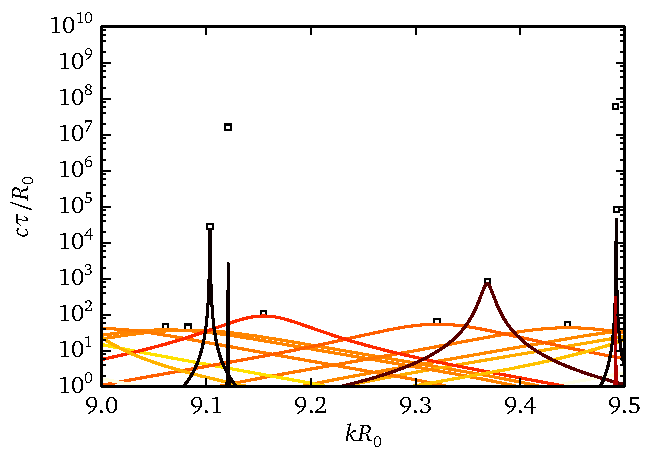
\includegraphics[width=0.8\textwidth]{figs/passive/correspondanceRootsPeaks.pdf}
  \caption[Correspondence between the poles of the scattering matrix and the peaks
	  of the time delay spectrum.]
	  {Time delay spectrum of a circular cavity with $n_c=3.2$ and $n_o=1$ in TM polarization. The squares
	  represent the complex position of the poles of the scattering matrix. The equivalent
	  time delay is computed using $c\tau/R_0=-\Re{kR_0}/2\Im{kR_0}$.}
  \label{fig:passive.numerical.correspondanceRoots}
\end{figure}


\begin{figure}
 \centering
 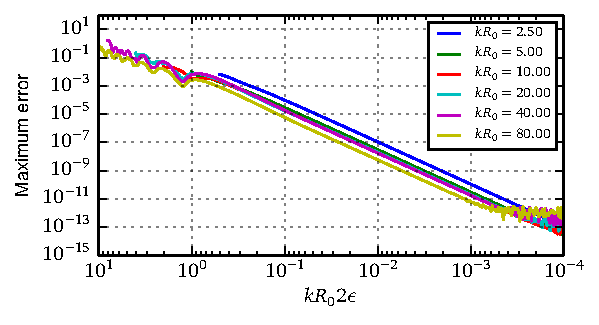
\includegraphics{figs/passive/convergenceHomo.pdf}
 \caption[Convergence properties of SQA when applied on the homogeneous disk]
	  {Calibration of \gls{sqa} against the homogeneous disk. The cavity 
	  has refractive index $n_c=1.5$ and is embedded in air $n_o=1$. The exterior
	  radius is set to $R_0=1$ and we take the number of shells to be $N=2$.
	  The error approximately follows a cubic power-law behaviour in the discretization
	  size.}
 \label{fig:passive.numerical.convergenceHomogeneousDisk}
\end{figure}

\paragraph{Annular Cavity}
The annular cavity is a circular cavity with constant refractive index
profile in which a circular hole has been cut, see Fig. \ref{fig:passive.numerical.annularCavityGeometry}
for a picture. 
Derivation of the scattering matrix of the annular cavity is a little
more involved. Suffice it to say that it is given by 
  \begin{equation}
   \mat{S}^\text{AC} = -\left[n_o{\mat{H}^{(-)}}'(Z_o)-n_c\mat{H}^{(-)}(Z_o)\mat{GF}^{-1}\right]
			\left[n_o{\mat{H}^{(+)}}'(Z_o)-n_c\mat{H}^{(+)}(Z_o)\mat{GF}^{-1}\right]^{-1}
  \end{equation}
where 
  \begin{align}
   \mat{F} &= \mat{H}^{(-)}(Z_c)+\mat{H}^{(+)}(Z_c)\mat{S}^\text{HD} & \mat{G} = {\mat{H}^{(-)}}'(Z_c)+{\mat{H}^{(+)}}'(Z_c)\mat{S}^\text{HD}.
  \end{align}
A proper derivation can be found in \cite{HEN2002b}; an improved
one can be found in \cite[Appendix D]{GAP2013a}.

\begin{figure}
  \begin{center}
  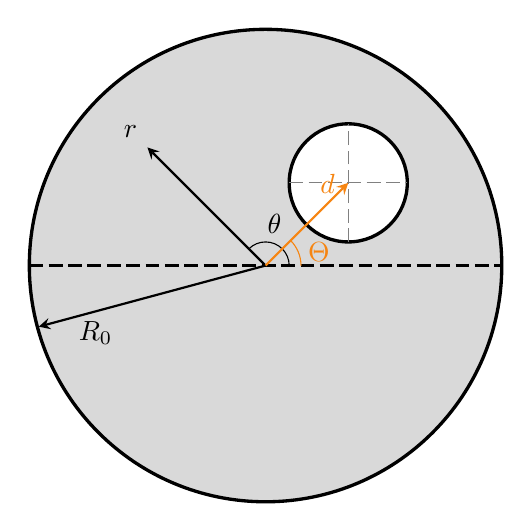
\begin{tikzpicture}[scale=3]
   % -- Draw basic geometry
   \draw[very thick,fill=gray!30!white] (0,0) circle (1);
   \draw[very thick,fill=white] (0.35,0.35) circle (0.25);
  
   % -- Draw coordinate systems and distances.
   % Center line.
   \draw[dash pattern=on 5pt off 2pt,thick] (-1,0) -- (1,0);
   
   % Coordinates of big cavity.
   \draw[->,>=stealth,thick] (0,0) -- (-0.5,0.5) node[above left] {$r$};
   \draw (0.1,0) arc (0:135:0.1) node[midway,above] {$\theta$};
   
   % Radius of big cavity.
   \draw[->,>=stealth,thick] (0,0) -- (-0.96,-0.2588) node[near end,below] {$R_0$};
   
   % Center lines for inclusion.
   \draw[dash pattern=on 5 pt off 2pt, gray] (0.1,0.35) -- (0.6,0.35);
   \draw[dash pattern=on 5 pt off 2pt, gray] (0.35,0.1) -- (0.35,0.6);
   
   % Coordinates of inclusion w/r to big cavity.
   \draw[->,>=stealth,thick,BurntOrange] (0,0) -- (0.35,0.35) node[near end, above] {$d$};
   \draw[BurntOrange] (0.15,0) arc (0:45:0.15) node[midway,right] {$\Theta$};
  \end{tikzpicture}
  \end{center}
  \caption[Geometry of the annular cavity]
	  {Geometry of the annular cavity. The circular cavity has coordinate system
	  $(r,\theta)$ and radius $R_0$ Its refractive index is denoted by $n_c$. 
	  The circular inclusion has position $\color{BurntOrange}(d,\Theta)$
	  in the main coordinates and its refractive index is $n_h$. It isually is the same
	  as $n_0$, the refractive index of the environment.}
  \label{fig:passive.numerical.annularCavityGeometry}
\end{figure}


\todo[inline]{Calibration with annular cavity.}

To make sure we can blindly accept the results of our numerical
technique, we apply it to non-integrable geometries that have been
studied by other means in the literature. Table \ref{tab:passive.numerical.comparisonLiterature}
shows a comparison of the positions of the certain resonances 
for a set of selected geometries. Fig. \ref{fig:passive.numerical.squareSpectrum}
shows the time delay spectrum of the square cavity. The higher-delay mode, 
highlighted in the figure, has a field profile (inset) that resembles
a WGM. The localization of light in square cavities has since been 
confirmed experimentally \cite{BIT2013} and observed in other geometries
\cite{SON2013}.

\begin{table}
  \newcolumntype{d}{D{.}{.}{3}}
  \begin{tabular*}{\columnwidth}{l@{\extracolsep{\fill}}ddddc}
  \hline\hline
  \multirow{2}{*}{Cavity}	& \multicolumn{2}{c}{SQA}					& \multicolumn{2}{c}{Emission Viewpoint}				& \multirow{2}{*}{Source}	\\
				& \multicolumn{1}{c}{$kR_0$}	& \multicolumn{1}{c}{$2R_0/c\tau$}	& \multicolumn{1}{c}{$\text{Re}\{kR_0\}$}&\multicolumn{1}{c}{$|\text{Im}\{kR_0\}|$}	&\\
\hline\hline
  Square			& 4.53				& \multicolumn{1}{c}{$1.06\times10^{-4}$}& 4.54					&\multicolumn{1}{c}{$1.05\times10^{-4}$}&\cite{GUO2003}\\
  Stadium			& 4.89				& 0.052					& 4.89					&0.055					&\cite{LEE2004}\\
  Ellipse			& 6.499				& 0.029					& 6.50					&0.032					&\cite{UNT2008}\\
  Annular			& 10.266			& 0.083					& 10.268				&0.081					&\cite{GAP2013a}\\
  \hline\hline
  \end{tabular*}
  \caption[Comparison of SQA results with results from the literature]
	  {Real and imaginary parts of the resonant frequencies computed with SQA compared
	  with results from the literature.}
  \label{tab:passive.numerical.comparisonLiterature}
\end{table}

\begin{figure}
 \centering
 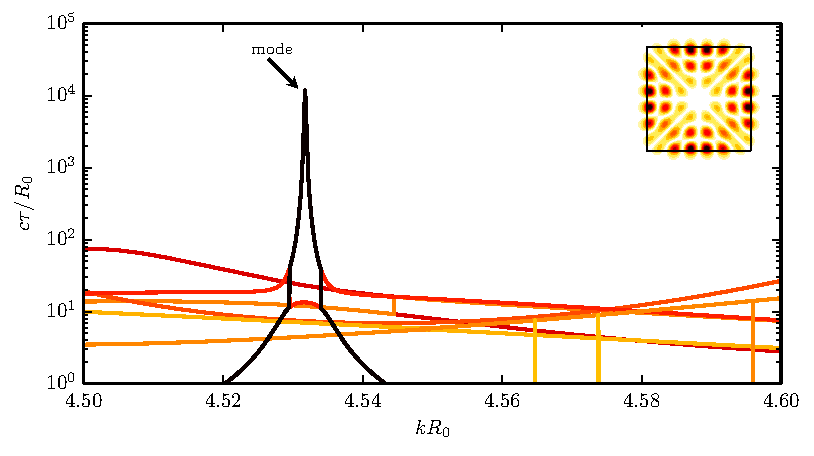
\includegraphics{figs/passive/spectrum_square_inset.pdf}
 \caption[Delay spectrum of the square cavity]
	 {Delay spectrum of the square cavity. The highlighted mode 
	 has a high $Q$-factor, which can be explained by its 
	 WGM-like field recirculation. The inset of the figure shows
	 the actual field profile of the mode. It was computed 
	 using COMSOL by G.P.-A. \cite{GAP2013a}.}
 \label{fig:passive.numerical.squareSpectrum}
\end{figure}

\section{Case Study: Gaussian Deformation of the Refractive Index}
As an academic demonstration of the power of the method, 
we present a study of a circular cavity whose refractive index
has a Gaussian shape
  \begin{equation}
   n(r,\theta) = n_0 + \delta n\exp\left[-\frac{r^2+2dr\cos\left(\Theta-\theta\right)+d^2}{2w^2}\right],
  \end{equation}
where $n_0$ is the background refractive index, $\delta _n$ the 
deformation amplitude, $w$ its half-width and $(d,\Theta)$
its position relative to the center of the cavity. 

As previously noted by G.~P-A. \cite{GAP2013a}, a peculiar
duality exists between high-$Q$ resonances and directional emission.
Working with a cavity similar to the annular one, it stands to reason
that we will recover the same pattern. This study will be used
as a stepping stone for our inquiries in the realm of non-uniformly
pumped active microcavities. 

\subsection{Loss of Integrability and the KAM Scenario}
When $d=0$, the potential is central and angular momentum is 
necessarily conserved. If the system is also unitary
(no absorption nor gain), it can be shown that the system is
integrable\footnote{The covariant form of Maxwell's equation and their
associated Euler-Lagrange equation make this conservation perfectly clear.}. 
This conservation of angular momentum in turn
implies circular symmetry of the fields and hence of the 
far-field radiation pattern. Since most applications (particularly lasers)
require a certain directionality in the emission, our goal is to break 
the circular symmetry in such a way as to minimize the degradation of the
finesse ($Q$-factor) and maximizing the output directionality. Historically, 
this goal has spawned the research field of \glspl{arc} wherein the boundary
of the circular cavity is parametrically deformed to yield limaçon, stadium, 
elliptical, quadrupolar, and other shapes. 

The underlying classical mechanics of \glspl{arc} follow the KAM scenario 
as the geometry is perturbed away from a perfect circle. In phase space, 
regularity yields to the chaotic sea, dividing it into regions of regular
motion and regions of ergodic motion. The Hamiltonian nature of the 
dynamics has been thoroughly studied and has been used to tame the 
animosity of directionality and high-$Q$ emission \cite{KWA2013,KIM2013}

In our case, we do not deform the boundary, leaving it a perfect circle, 
but use a deformation of the refractive index. This particular deformation
-- the Gaussian one -- 
is of theoretical and practical interest, as it can easily be induced
by shining light on the dielectric from above. This refractive
index profile is also obtained when pumping a microcavity laser
with another laser.

\subsection{Numerical Results}
Fig.~\ref{fig:passive.gaussian.numericalResults.farField} shows our primary
result, i.e. that loss of symmetry may introduce directionality
in the far-field. The directionality is mild in our example, but the 
cavity serves as a proof-of-concept. In Fig.~\ref{fig:passive.gaussian.numericalResults.spectrum}, 
the dotted blue lines show the delay spectrum of the centered Gaussian (CG) deformation, 
an integrable cavity, and the full red lines the spectrum of the non-centered Gaussian
(NG) deformation. Notice that the higher-delay modes are barely affected by 
the inhomogeneity. While we do not know the field profile\todo{Compute field with integral method.}, 
it is safe to assume the two high-delay modes behave like WGMs. Although it is not shown, 
both modes have isotropic far-fields. The rather small shift in wavenumber can be
understood by the slight rarefaction of the medium near the deformation. 
The field must ``evade'' being caught by the deformation to retain
its WGM properties, which results in slight positive increase in $k$ (smaller wavelength). 

\begin{figure}
 \centering
 \begin{subfigure}{0.6\textwidth}
  \centering
  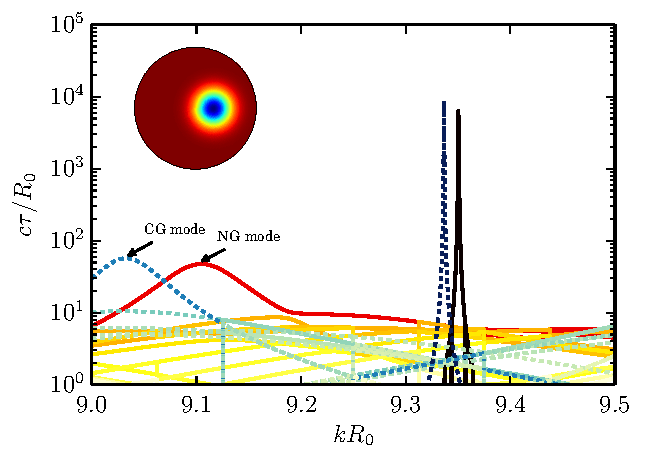
\includegraphics[width=\textwidth]{figs/passive/spectrum_gaussian_inset.pdf}
  \caption[Delay spectrum of the Gaussian microcavity]
	  {Delay spectrum of the gaussian microcavity. The dotted blue lines show the spectrum
	  for the integrable case of the deformation, i.e. $d=\Theta=0$ (CG mode). The full red lines
	  show the spectrum for the deformation centered at $d=0.3R_0$ and $\Theta=0$ (NG mode).}
  \label{fig:passive.gaussian.numericalResults.spectrum}
 \end{subfigure}
 \begin{subfigure}{0.39\textwidth}
  \centering
  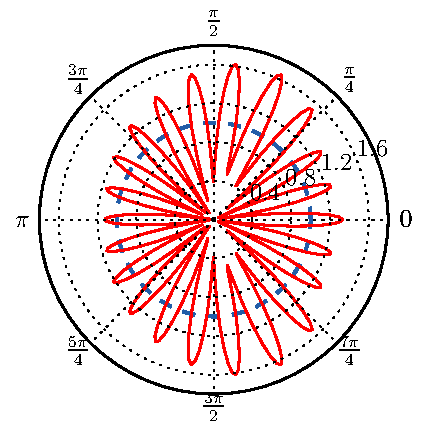
\includegraphics[width=\textwidth]{figs/passive/farField_gaussian.pdf}
  \caption{Far-fields of both CG (dotted blue) and NG (full red) modes. The isotropy is broken 
	  when the potential loses its circular symmetry. The NG mode has mild directionality
	  in the directions $\theta=\pm65^\circ$, owing to the diverging lens effect of the deformation.}
  \label{fig:passive.gaussian.numericalResults.farField}
 \end{subfigure}
 \caption[Delay spectrum of the Gaussian cavity and the far-fields of two chosen modes]
	  {Delay spectrum and far-field. \textbf{\subref{fig:passive.gaussian.numericalResults.spectrum}} 
	  Delay spectrum of cavity with the Gaussian deformation with parameters $n_0=2$, $\delta n=-1$ and $w=0.2R_0$.
	  \textbf{\subref{fig:passive.gaussian.numericalResults.farField}} shows the far-field of the both the CG and NG modes.
	  Notice the mild directionality of the NG mode.}
 \label{fig:passive.gaussian.numericalResults}
\end{figure}

The lower delay modes, the highlighted ones in \ref{fig:passive.gaussian.numericalResults.spectrum}
are more affected by the inhomogeneity, as their field must be more
extended in the dielectric. The field thus ``feels'' a greater
rarefaction of the medium and the mode suffers both a greater $\Delta k$
and a pronounced change in its emission properties. The angular momentum
mixing is such that that the ``backscattering'' $|\psi_\text{FF}(\theta=\pi)|$
is minimized and that the scattering in directions $\theta\sim\pm3\pi/8$
is favoured. This directionality may somewhat be explained by a
ray analysis of the system, as the deformation acts as a diverging
lens. The next section will explain this in more detail. 

\subsection{Geodesics and Ray Analysis\footnote{We use Schutz's \cite{SCH2009} notation in this section.
Repeated indices are summed over; $g_{\alpha\beta}$ is the metric tensor; the notation 
$M_{\alpha\beta,\gamma}$ indicates differentiation with respect to $\gamma$. The contravariant
tensor $g^{\alpha\beta}$ is the inverse of $g_{\alpha\beta}$, i.e. $g^{\alpha\beta}g_{\beta\gamma}={\delta^\alpha}_\gamma$}.}
While our numerical method allows us tu perform full-wave
simulations of cavities, it is often useful to consider the associated
billiard system, which is the small wavelength approximation of 
Helmholtz's equation. In homogeneous ARCS, photons follow straight path
trajectories and are specularly reflected at the interfaces. In inhomogeneous
\glspl{arc}, photons follow curved trajectories that obey Fermat's principle. 
The general equations defining those \textit{geodesic} paths can be found
by using the metric
  \begin{equation}
   (dt)^2=g_{\mu\nu}dx^\mu dx^\nu. 
  \end{equation}
For photons, the metric is simply given by the optical length 
of the medium, $g_{\mu\nu}=n^2(\bo{r})\delta_{\mu\nu}$. 
The time it takes to travel a particular trajectory is given by
  \begin{equation}
   t = \int_{\lambda_0}^{\lambda_1} \sqrt{g_{\mu\nu}\dot{x}^\mu\dot{x}^\nu}\,d\lambda
  \end{equation}
where $\lambda$ is a parameter of the curve. By Fermat's principle, photon 
trajectories minimize the time of flight. We thus apply the Euler-Lagrange
equation 
  \begin{align}
   \frac{\partial L}{\partial x^\alpha}-\frac{d}{d\lambda}\frac{\partial L}{\partial\dot{x}^\alpha}=0
  \end{align}
on the functional $L=\sqrt{w}=\sqrt{g_{\mu\nu}\dot{x}^\mu\dot{x}^\nu}\,d\lambda$ Evaluating the derivatives
  \begin{align*}
  0	&=\frac{\partial\left(\sqrt{w}\right)}{\partial x^\alpha}-\frac{d}{d\lambda}\frac{\partial\left(\sqrt{w}\right)}{\partial\dot{x}^\alpha}	\\
  {}	&=\frac{\partial w}{\partial x^\alpha}+\frac{1}{2\sqrt{w}}\frac{dw}{d\lambda}\frac{\partial w}{\partial\dot{x}^\alpha}-\frac{d}{d\lambda}\frac{\partial w}{\partial\dot{x}^\alpha}
  \end{align*}
When $\lambda$ is an affine parameter, the derivative $dw/d\lambda$ vanishes \cite{TOP2005,SCH2009}
and the Euler-Lagrange equation becomes
  \begin{align*}
  \frac{\partial w}{\partial x^\alpha}			&= \frac{d}{d\lambda}\frac{\partial w}{\partial\dot{x}^\alpha}	\\
  g_{\mu\nu,\alpha}\dot{x}^\mu\dot{x}^\nu		&= \frac{d}{d\lambda}\left[g_{\mu\nu}{\delta_\alpha}^\mu\dot{x}^\nu+g_{\mu\nu}{\delta_\alpha}^\nu\dot{x}^\mu\right]	\\
							&= \frac{d}{d\lambda}\left[g_{\alpha\nu}\dot{x}^\nu+g_{\mu\alpha}\dot{x}^\mu\right]					\\
							&= g_{\alpha\nu,\lambda}\dot{x}^\lambda\dot{x}^\nu+g_{\alpha\nu}\ddot{x}^\nu+g_{\mu\alpha,\lambda}\dot{x}^\lambda\dot{x}^\mu+g_{\mu\alpha}\ddot{x}^\mu \tag{chain rule: $\frac{dg_{\mu\nu}}{d\lambda}=\frac{\partial g_{\mu\nu}}{\partial x^\lambda}\frac{dx^\lambda}{d\lambda}$}	\\
  g_{\alpha\nu}\ddot{x}^\nu+g_{\mu\alpha}\ddot{x}^\mu	&= \dot{x}^\mu\dot{x}^\nu\left[g_{\mu\nu,\alpha}-g_{\alpha\nu,\mu}-g_{\mu\alpha,\nu}\right]	\tag{collecting differentiation orders}	\\
  {\delta^\sigma}_\mu\ddot{x}^\mu			&= \frac{1}{2}g^{\sigma\alpha}\left[g_{\mu\nu,\alpha}-g_{\alpha\nu,\mu}-g_{\alpha\mu,\nu}\right]\dot{x}^\mu\dot{x}^\nu	\tag{symmetry of $g_{\mu\nu}$ and $\times g^{\sigma\alpha}$}
  \end{align*}
This finally yields the equation
  \begin{equation}
   \ddot{x}^\sigma + {\Gamma^\sigma}_{\mu\nu}\dot{x}^\mu\dot{x}^\nu=0
  \end{equation}
where ${\Gamma^\sigma}_{\mu\nu}$ are the Christoffel symbols of the second kind. 

This last equation describes the trajectories of classical photons in any media. 
At interfaces, where the optical parameters have a jump discontinuity, one must use
Fresnel's laws, and possibly their generalization for curved interfaces \cite{HEN2002a}.

We will now obtain the equations for our Gaussian deformation. The author of this essay
would have expected that an analytical solution be available for the central Gaussian
potential, but the non-linearity of the equations spoil the symmetry and the hopes 
of finding a solution. We will thus solve the equations in Cartesian coordinates
for the centered formation:
  \begin{equation}
   n(x,y) = n_0 + \delta n \exp\left[-\frac{x^2+y^2}{2w^2}\right].
  \end{equation}
In Cartesian coordinates, the six independent Christoffel symbols have
value
  \begin{align*}
   {\Gamma^x}_{xx}			&= \frac{n_x}{n}	&	{\Gamma^y}_{xx}	&=-\frac{n_y}{n}\\
   {\Gamma^x}_{xy}={\Gamma^x}_{yx} 	&= \frac{n_y}{n}	&	{\Gamma^y}_{xy}={\Gamma^y}_{yx}&=\frac{n_x}{n}\\
   {\Gamma^x}_{yy}			&= -\frac{n_x}{n}	&	{\Gamma^y}_{yy}	&=\frac{n_y}{n}
  \end{align*}
which yield the equations
  \begin{subequations}
  \begin{align}
   \ddot{x}	&= \frac{x/w^2}{1+\frac{n_0}{\delta n}\exp\left[\frac{x^2+y^2}{2w^2}\right]}\left(\dot{x}^2-\dot{y}^2\right)
	    +\frac{2y/w^2}{1+\frac{n_0}{\delta n}\exp\left[\frac{x^2+y^2}{2w^2}\right]}\dot{x}\dot{y}				\\
   \ddot{y}	&= \frac{y/w^2}{1+\frac{n_0}{\delta n}\exp\left[\frac{x^2+y^2}{2w^2}\right]}\left(\dot{y}^2-\dot{x}^2\right)
		  +\frac{2x/w^2}{1+\frac{n_0}{\delta n}\exp\left[\frac{x^2+y^2}{2w^2}\right]}\dot{x}\dot{y}.
  \end{align}
  \end{subequations}
We seperate the two second-order equations in four first-order equations by defining $p_x=\dot{x}$ and $p_y=\dot{y}$. 
We solve the equations for photons coming in from $x(0)\rightarrow-\infty$ with $p_x(0)=\text{const}$
and $p_y(0)=0$ for different values of the impact parameters $y(0)=b$. The results are shown in 
Fig.~\ref{fig:passive.gaussian.geodesics} and from this simple analysis we see that 
the deformation acts as a diverging lens. 
\begin{figure}
 \centering
 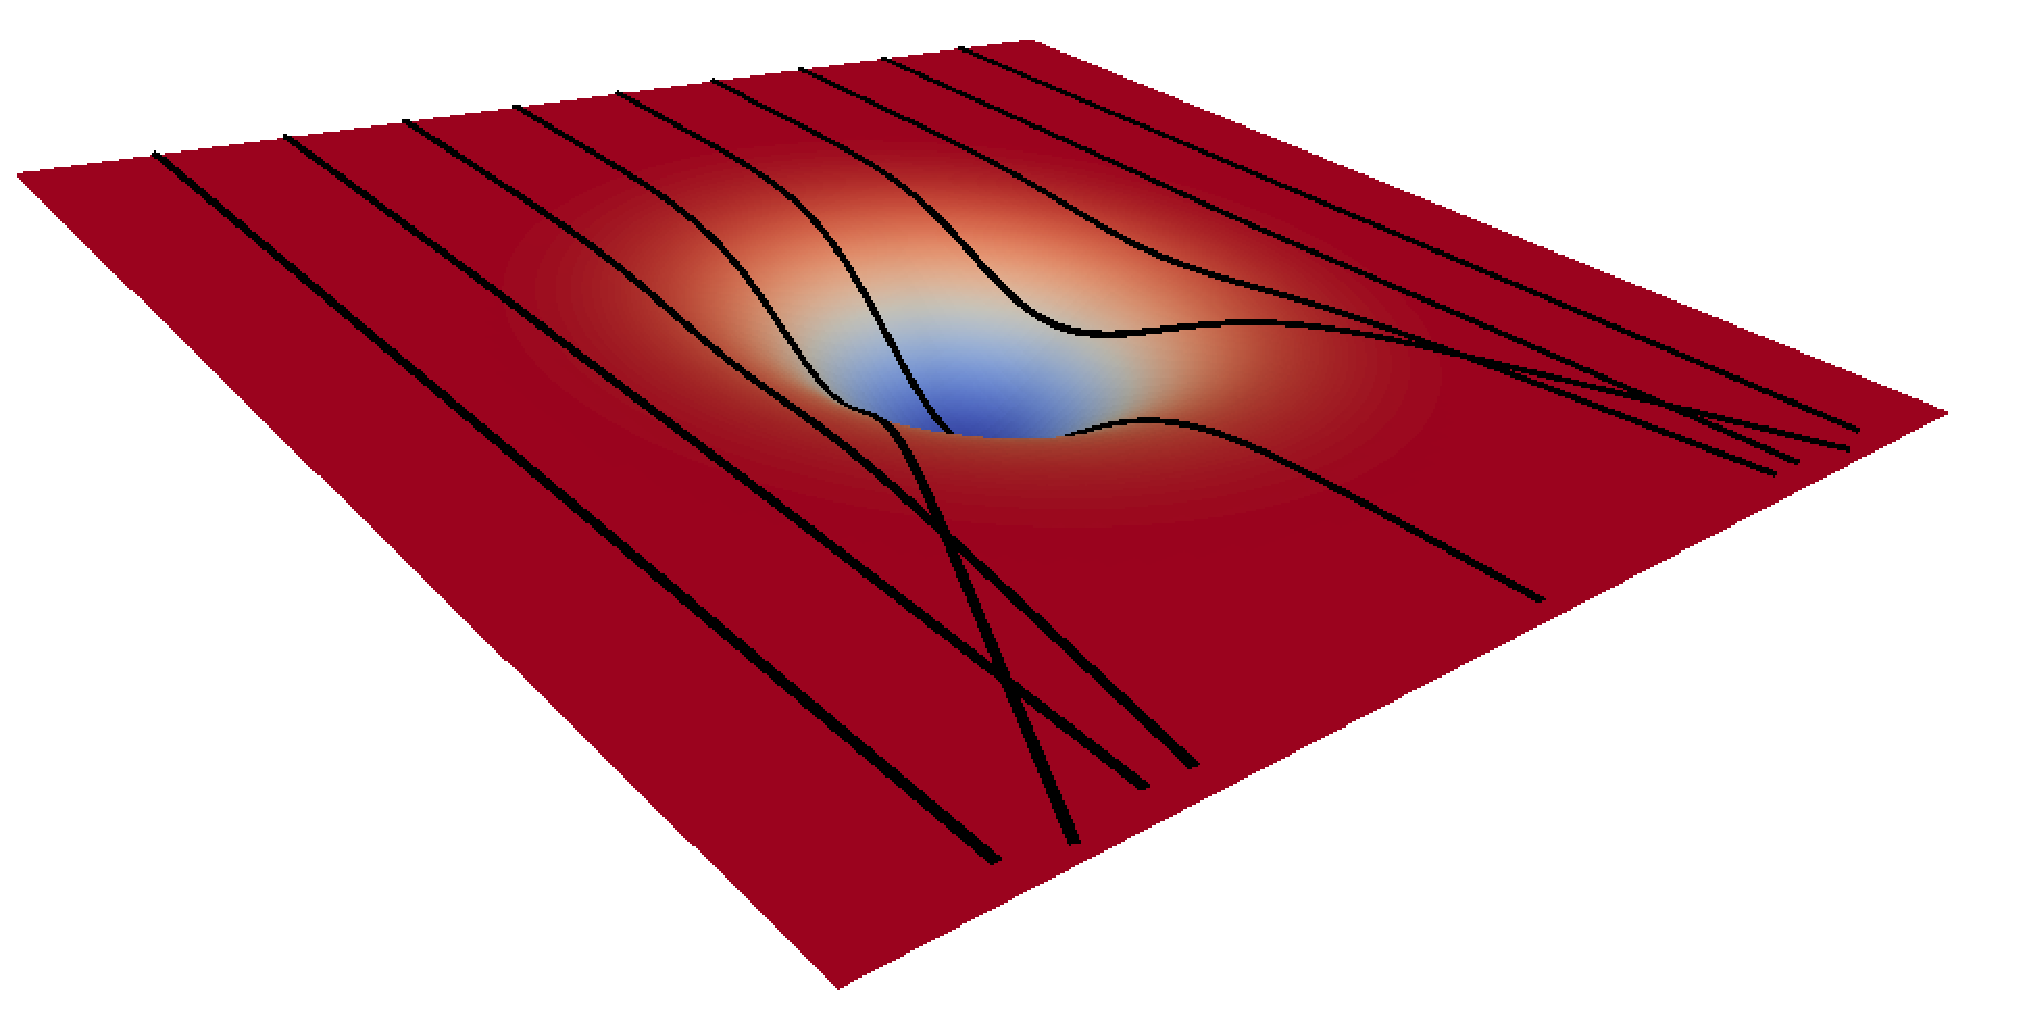
\includegraphics[width=0.75\textwidth]{figs/passive/geodesics-1.eps}
 \caption[Photon trajectories in a Gaussian deformation of the refractive index]
	  {Trajectories for photons of different impact parameters. The trajectories are
	  the geodesics of the relevant ``optical spacetime'', where the curvature of 
	  space represents the optical distance that the photon has to traverse. The central
	  region, where the refractive index is lower, acts as a diverging lens.}
 \label{fig:passive.gaussian.geodesics}
\end{figure}

From these equations, a more sophisticated algorithm could be developed to study
the associated classical mechanics of inhomogeneous billiard systems, as was done
in \cite{SAI2005}. The algorithm would need to include collision detection with the 
boundary of the billiard as well as formulas for the reflection and transmission coefficients
at this boundary.

\section{Conclusion and Perspectives}
This section solved the scattering problem of bidimensional
dielectric cavities. Using information on the real $k$-line,
the \gls{qMatrix} allows for the computation of the complex poles
of the scattering matrix, which in turn correspond to the resonances
of the scatterer. The eigenvectors of the \gls{qMatrix} define 
a set of modes that exist each real value of $k$. The eigenvectors
which correspond to peaks in the time delay spectrum can be associated
with the complex poles of $\mat{S}(k)$.

The formalism is coupled to a numerical method that computes 
the scattering matrix for inhomogeneous bidimensional cavities.
The method is based on an onion-like discretization scheme
where the solution of Helmholtz's equation can be reduced to an 
eigenvalue problem. This leads to the construction of local, or 
``shell scattering matrices''. The boundary conditions allow to fuse
the shells of the onion and compute the effect of the whole scatterer, 
viz. the scattering matrix.

The method is fast enough that it is possible to consider
an optimization problem with one or several cost functions
that quantify the performance of the scatterer for a
given application. A few examples spring to mind, such as
a dielectric optical switch, beam splitters, biosensors and others. 
If the material is active, one cold optimize the form of the pump 
profile to minimize thresholds and maximizing, for instance, output
directionality and power. 

One subject we have failed to mention in the main text is the 
fragility of the generalization of the \gls{sqa} to complex
energies $k$ and potentials $n$; it also becomes computationally
heavy. The details of the fragility are discussed in Appendix
\ref{sec:app.numTools.scatMat}. This, coupled to the instabilities
related to the reconstruction of the field inside the scatterer
has been a motivation to look for other numerical methods. In 
the next chapter, we will develop an \textit{integral} method
for the computation of the scattering matrix. This flexible
method will be use of great use in discussing active material 
and 3D geometries. 

% %From the general to the specific, scattering methods to solve
% %Maxwell's equations. 
% 
% \begin{itemize}
%  \item Lippmann-Schwinger type method. 
%   \begin{itemize}
%     \item Allows for full control over discretization. 
%     \item Takes Sommerfeld radiation condition into account analytically.
%     \item Must perform solution of vectorial 3D Fredholm equation. 
%   \end{itemize}
%  \item SQA
%   \begin{itemize}
%     \item Derivation of equations.
%       \begin{itemize}
% 	\item Effective Index Approximation and $\beta=0$.
% 	\item TM + TE polarizations.
%       \end{itemize}
%     \item Generalization of method to complex $n$.
%       \begin{itemize}
% 	\item Dual basis. 
% 	\item Numerical analysis of algorithm.
%       \end{itemize}
%     \item Difficulty: Field reconstruction. 
%   \end{itemize}
%  \item Variable Phase Method
%   \begin{itemize}
%     \item Derivation for 2D (3D?)
%     \item Results
%   \end{itemize}
%   
% \end{itemize}
